% Este apéndice proporciona información complementaria para reforzar la solución
% propuesta sin sobrecargar el cuerpo principal del paper.
% - Especificaciones de software y hardware requeridas.
% - Diagramas de arquitectura del sistema LMS.
% - Algoritmos utilizados para personalizar el microaprendizaje.
% - Capturas de pantalla o ejemplos de la interfaz del LMS.
% - Resultados detallados de pruebas piloto o estudios de usabilidad.
% - Comparación con otros LMS tradicionales y sus limitaciones.
% - Formularios utilizados para evaluar la efectividad del sistema.
% - Respuestas clave de usuarios o docentes sobre la experiencia de aprendizaje.
% - Segmentos relevantes del código para la implementación del LMS.
% - Scripts utilizados para la automatización de contenido microlearning.
% - Fórmulas aplicadas en la recomendación de contenidos.
% - Estadísticas detalladas sobre mejora en el aprendizaje.
% - Glosario de términos técnicos utilizados.
% - Documentación técnica adicional.

% La opción [H] en \begin{figure}[H] proviene del paquete float y significa ''Colocar la figura exactamente aquí''.

\appendices
\section{Interfaz del Sistema en Imágenes}

\begin{figure}[H]
    \centering
    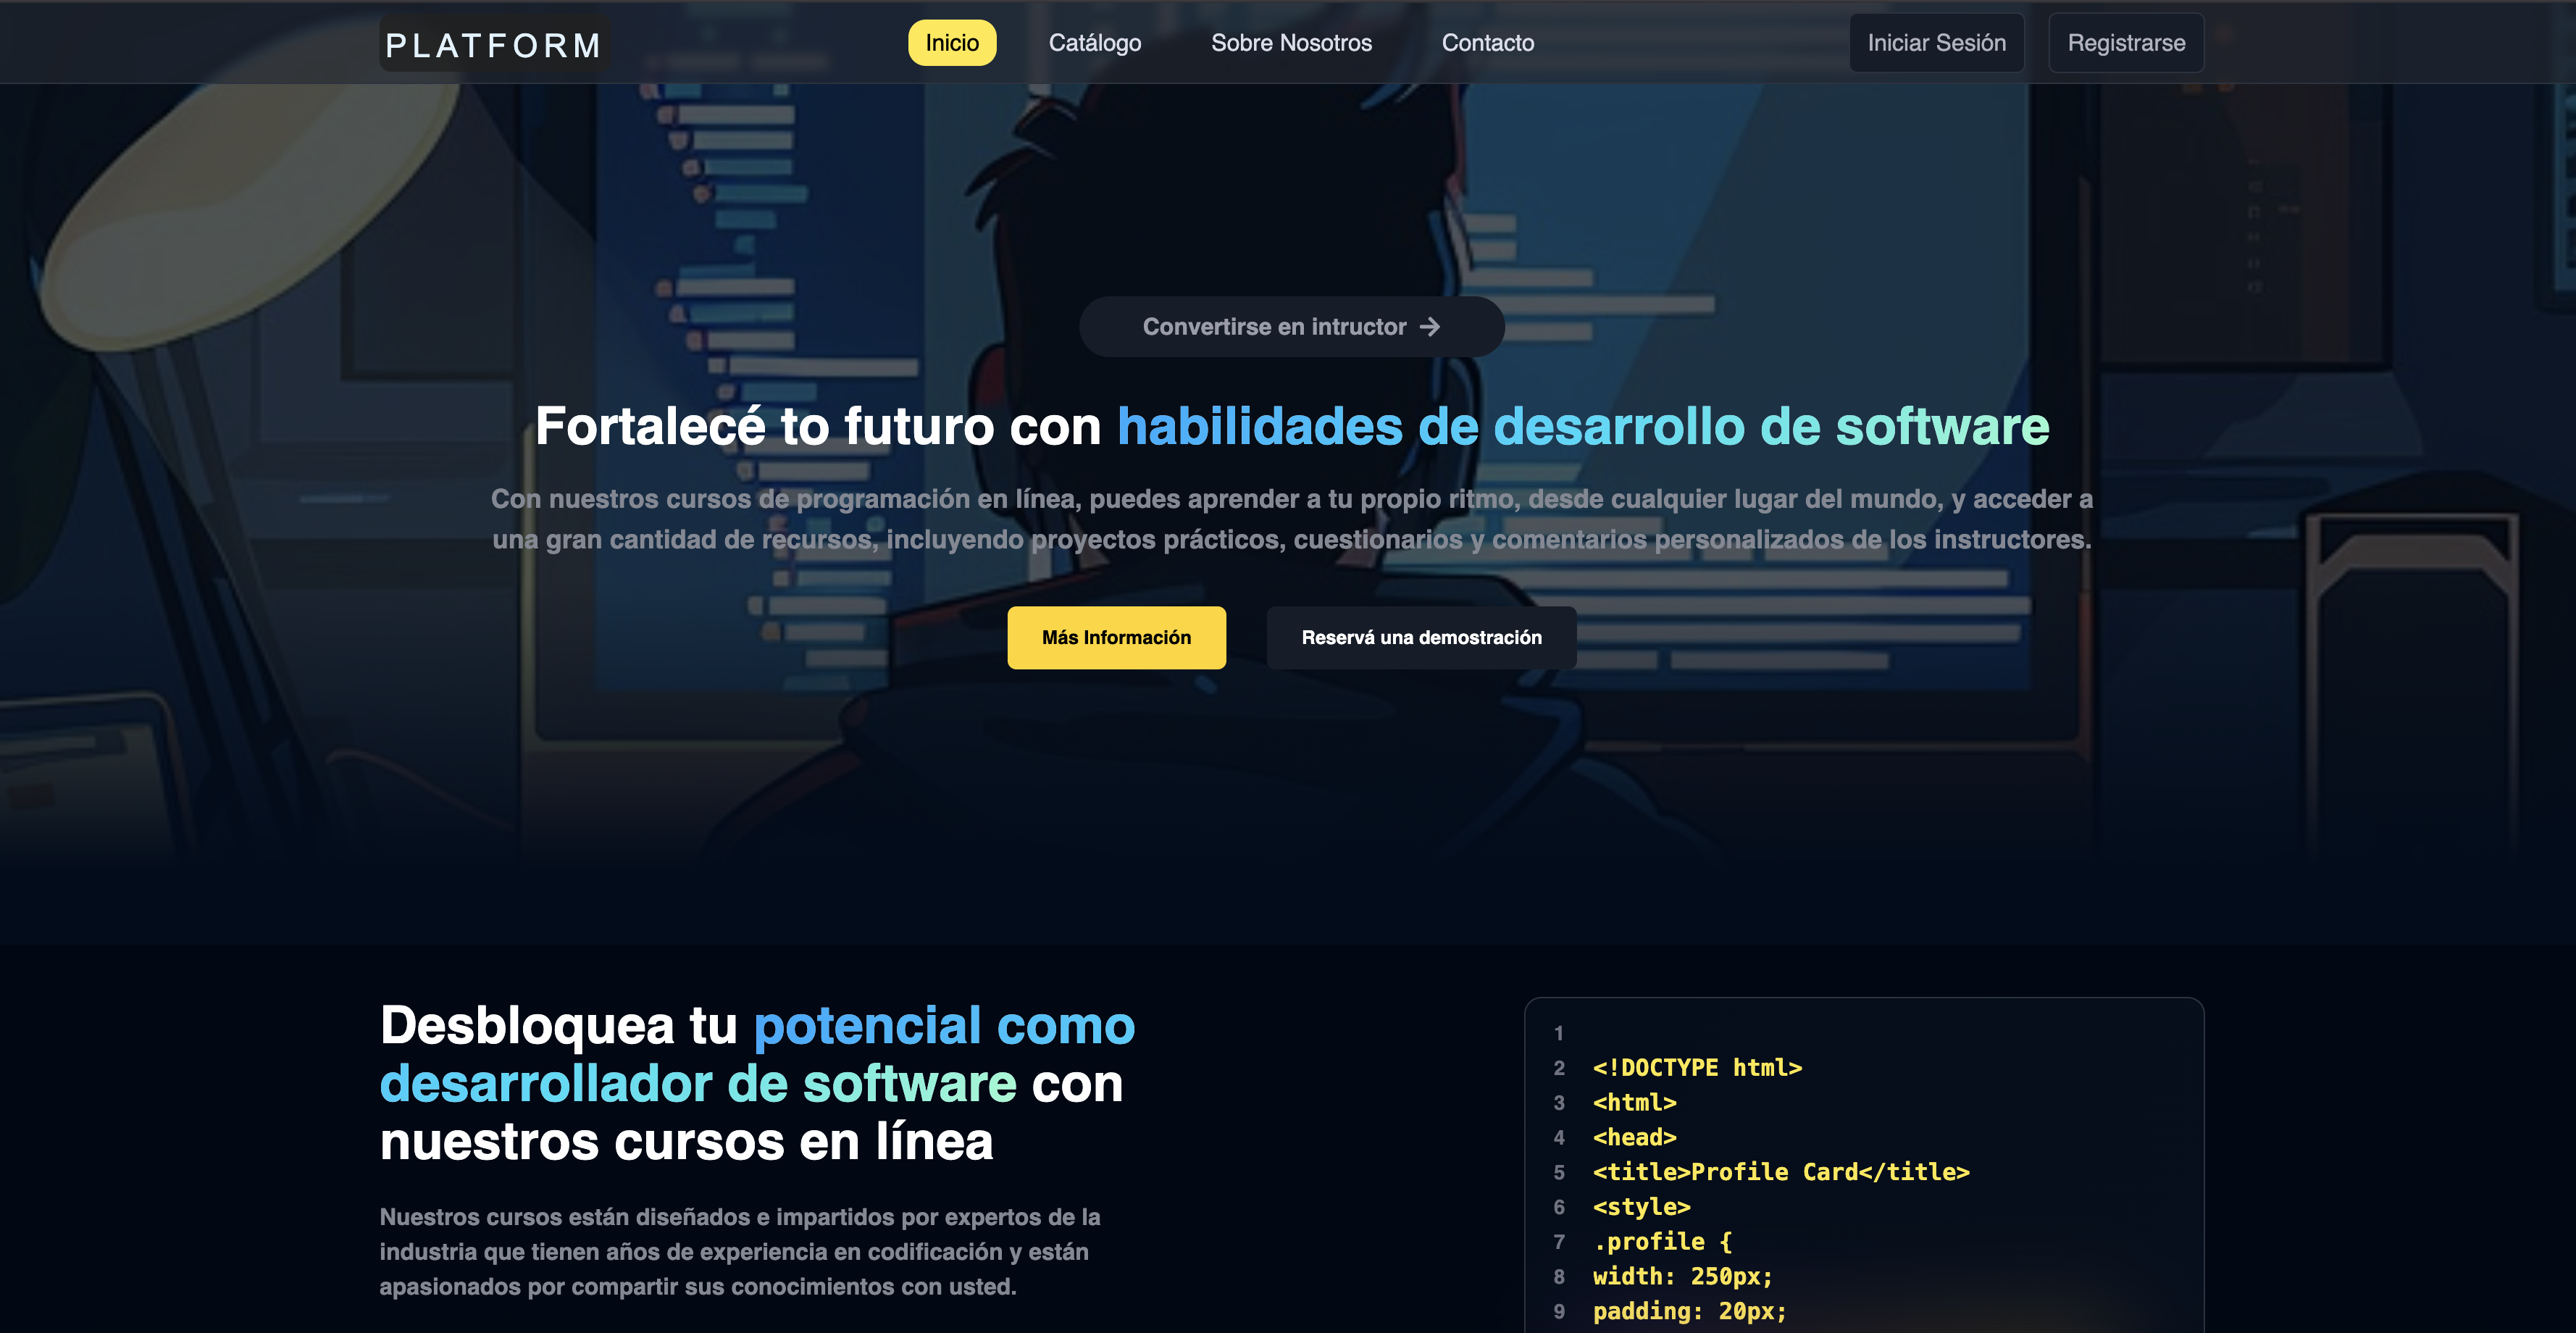
\includegraphics[width=\linewidth]{plataforma/plataforma_01.png}
    \caption{Interfaz de la página de inicio}
    \label{fig:interfaz_sistema_pagina_inicio}
\end{figure}

\begin{figure}[H]
    \centering
    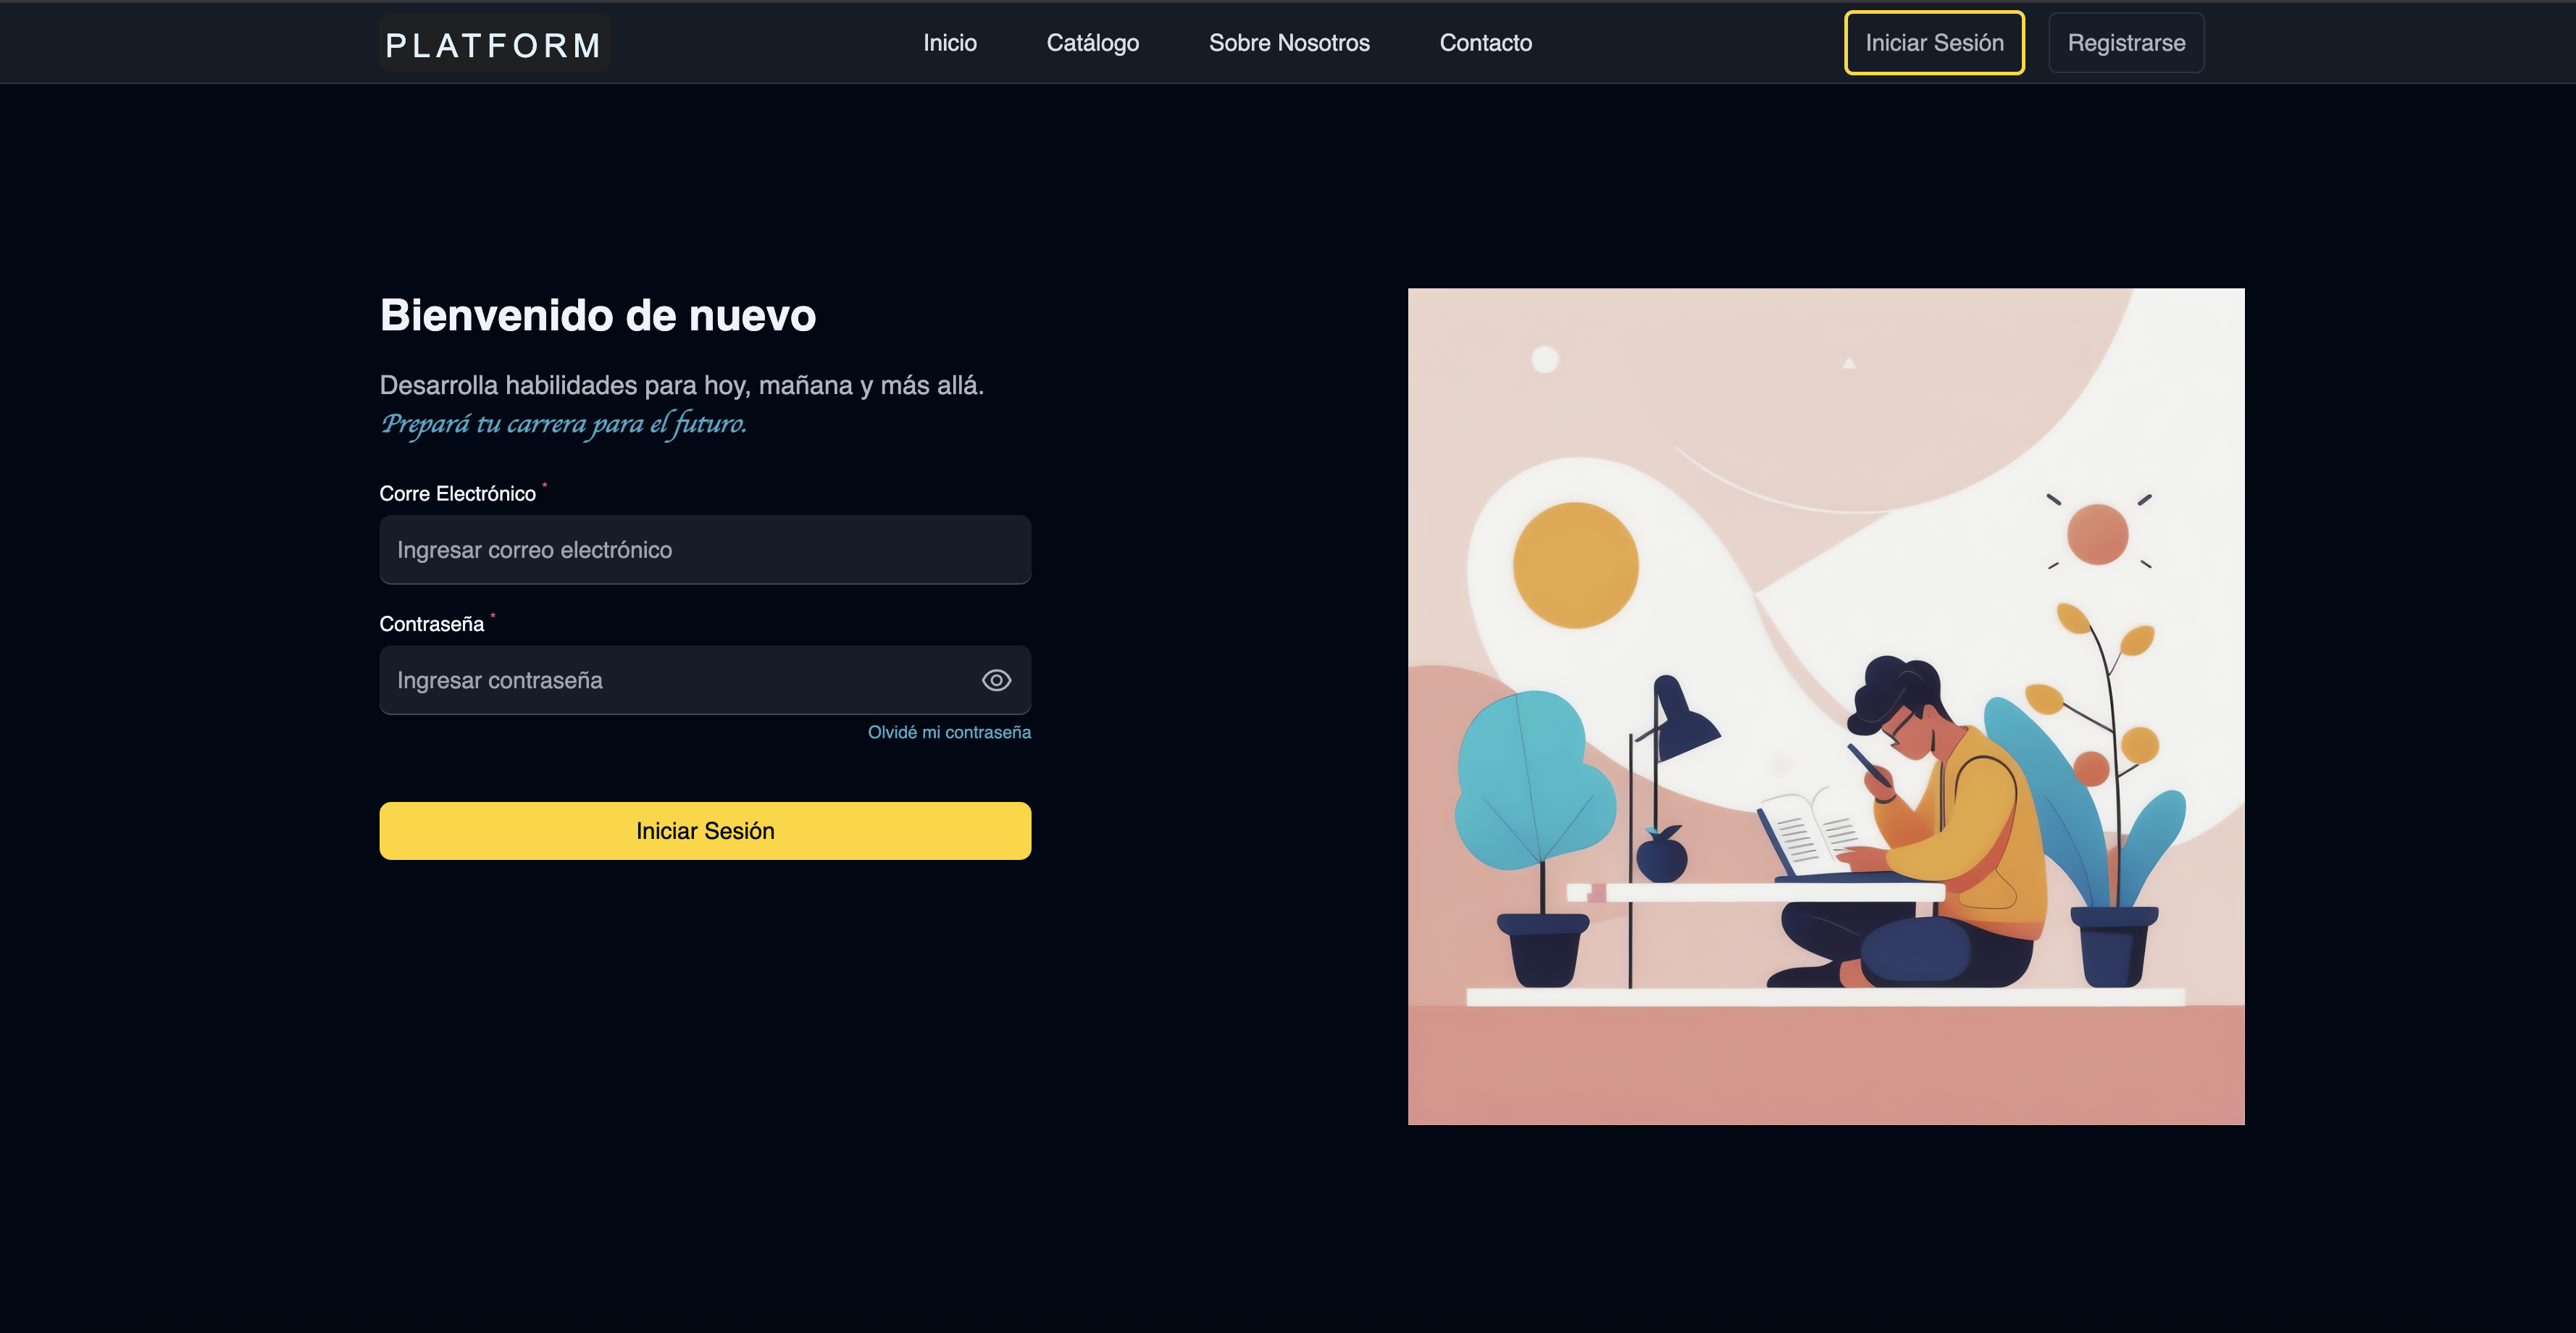
\includegraphics[width=\linewidth]{plataforma/plataforma_02.png}
    \caption{Interfaz de inicio de sesión}
    \label{fig:interfaz_sistema_inicio_sesión}
\end{figure}

\begin{figure}[H]
    \centering
    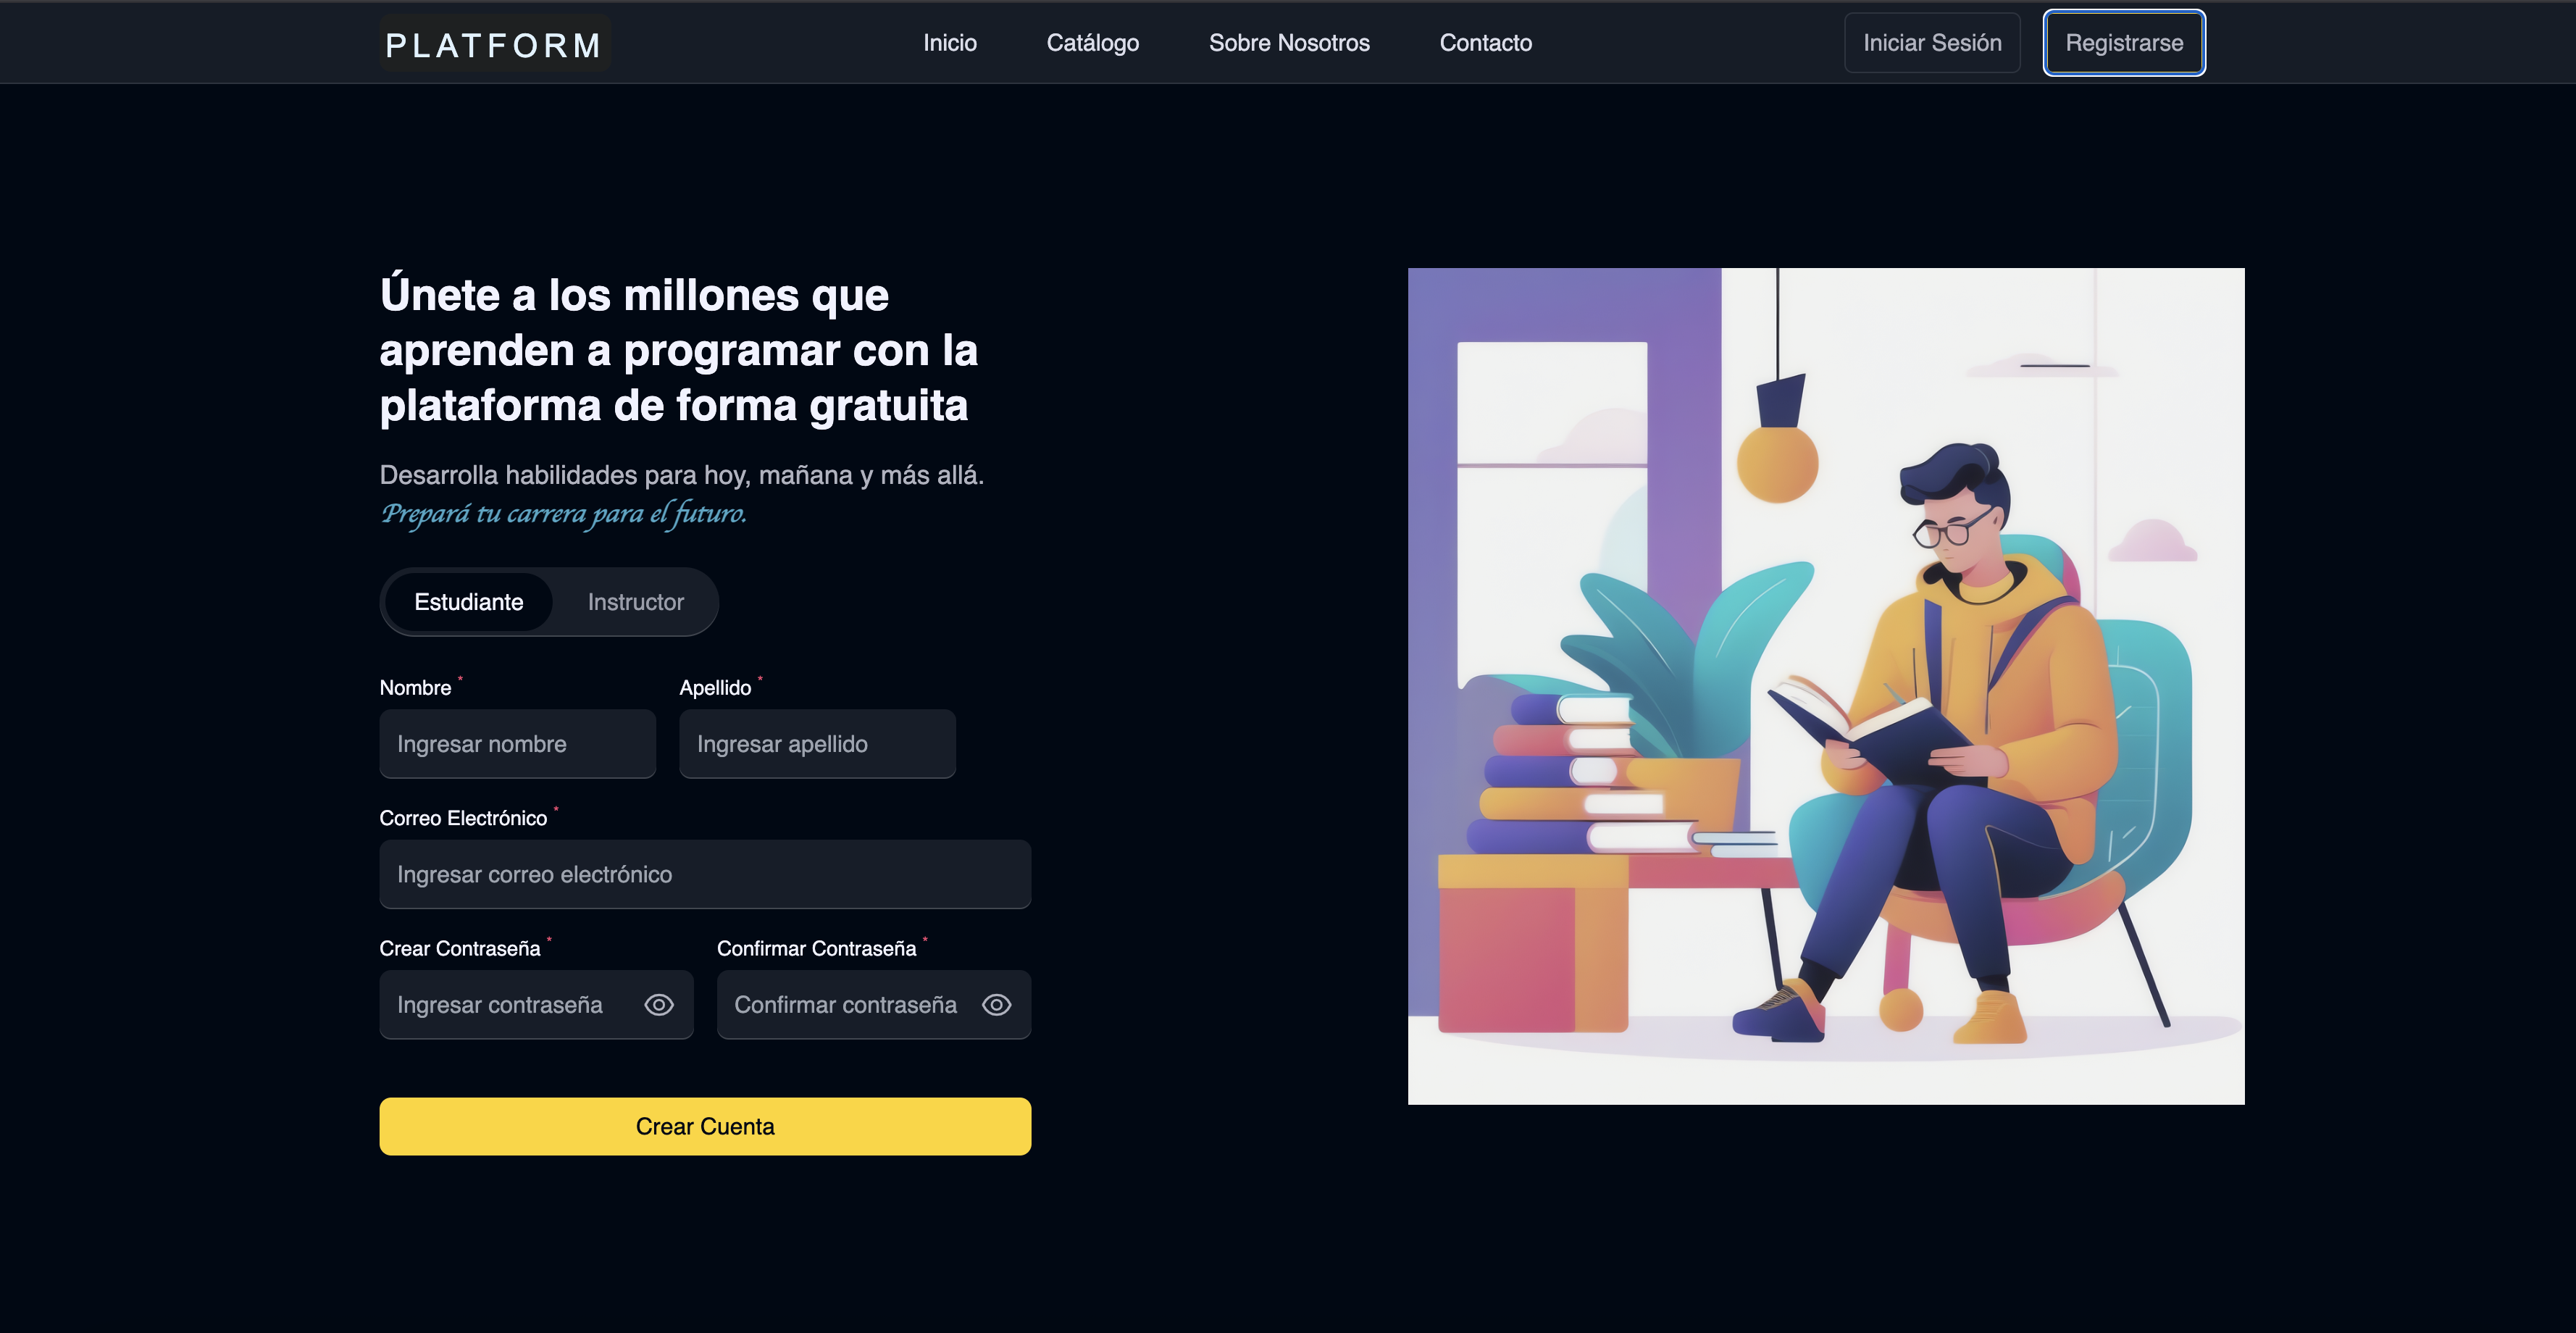
\includegraphics[width=\linewidth]{plataforma/plataforma_03.png}
    \caption{Interfaz del registro de usuario}
    \label{fig:interfaz_sistema_registro_usuario}
\end{figure}

\begin{figure}[H]
    \centering
    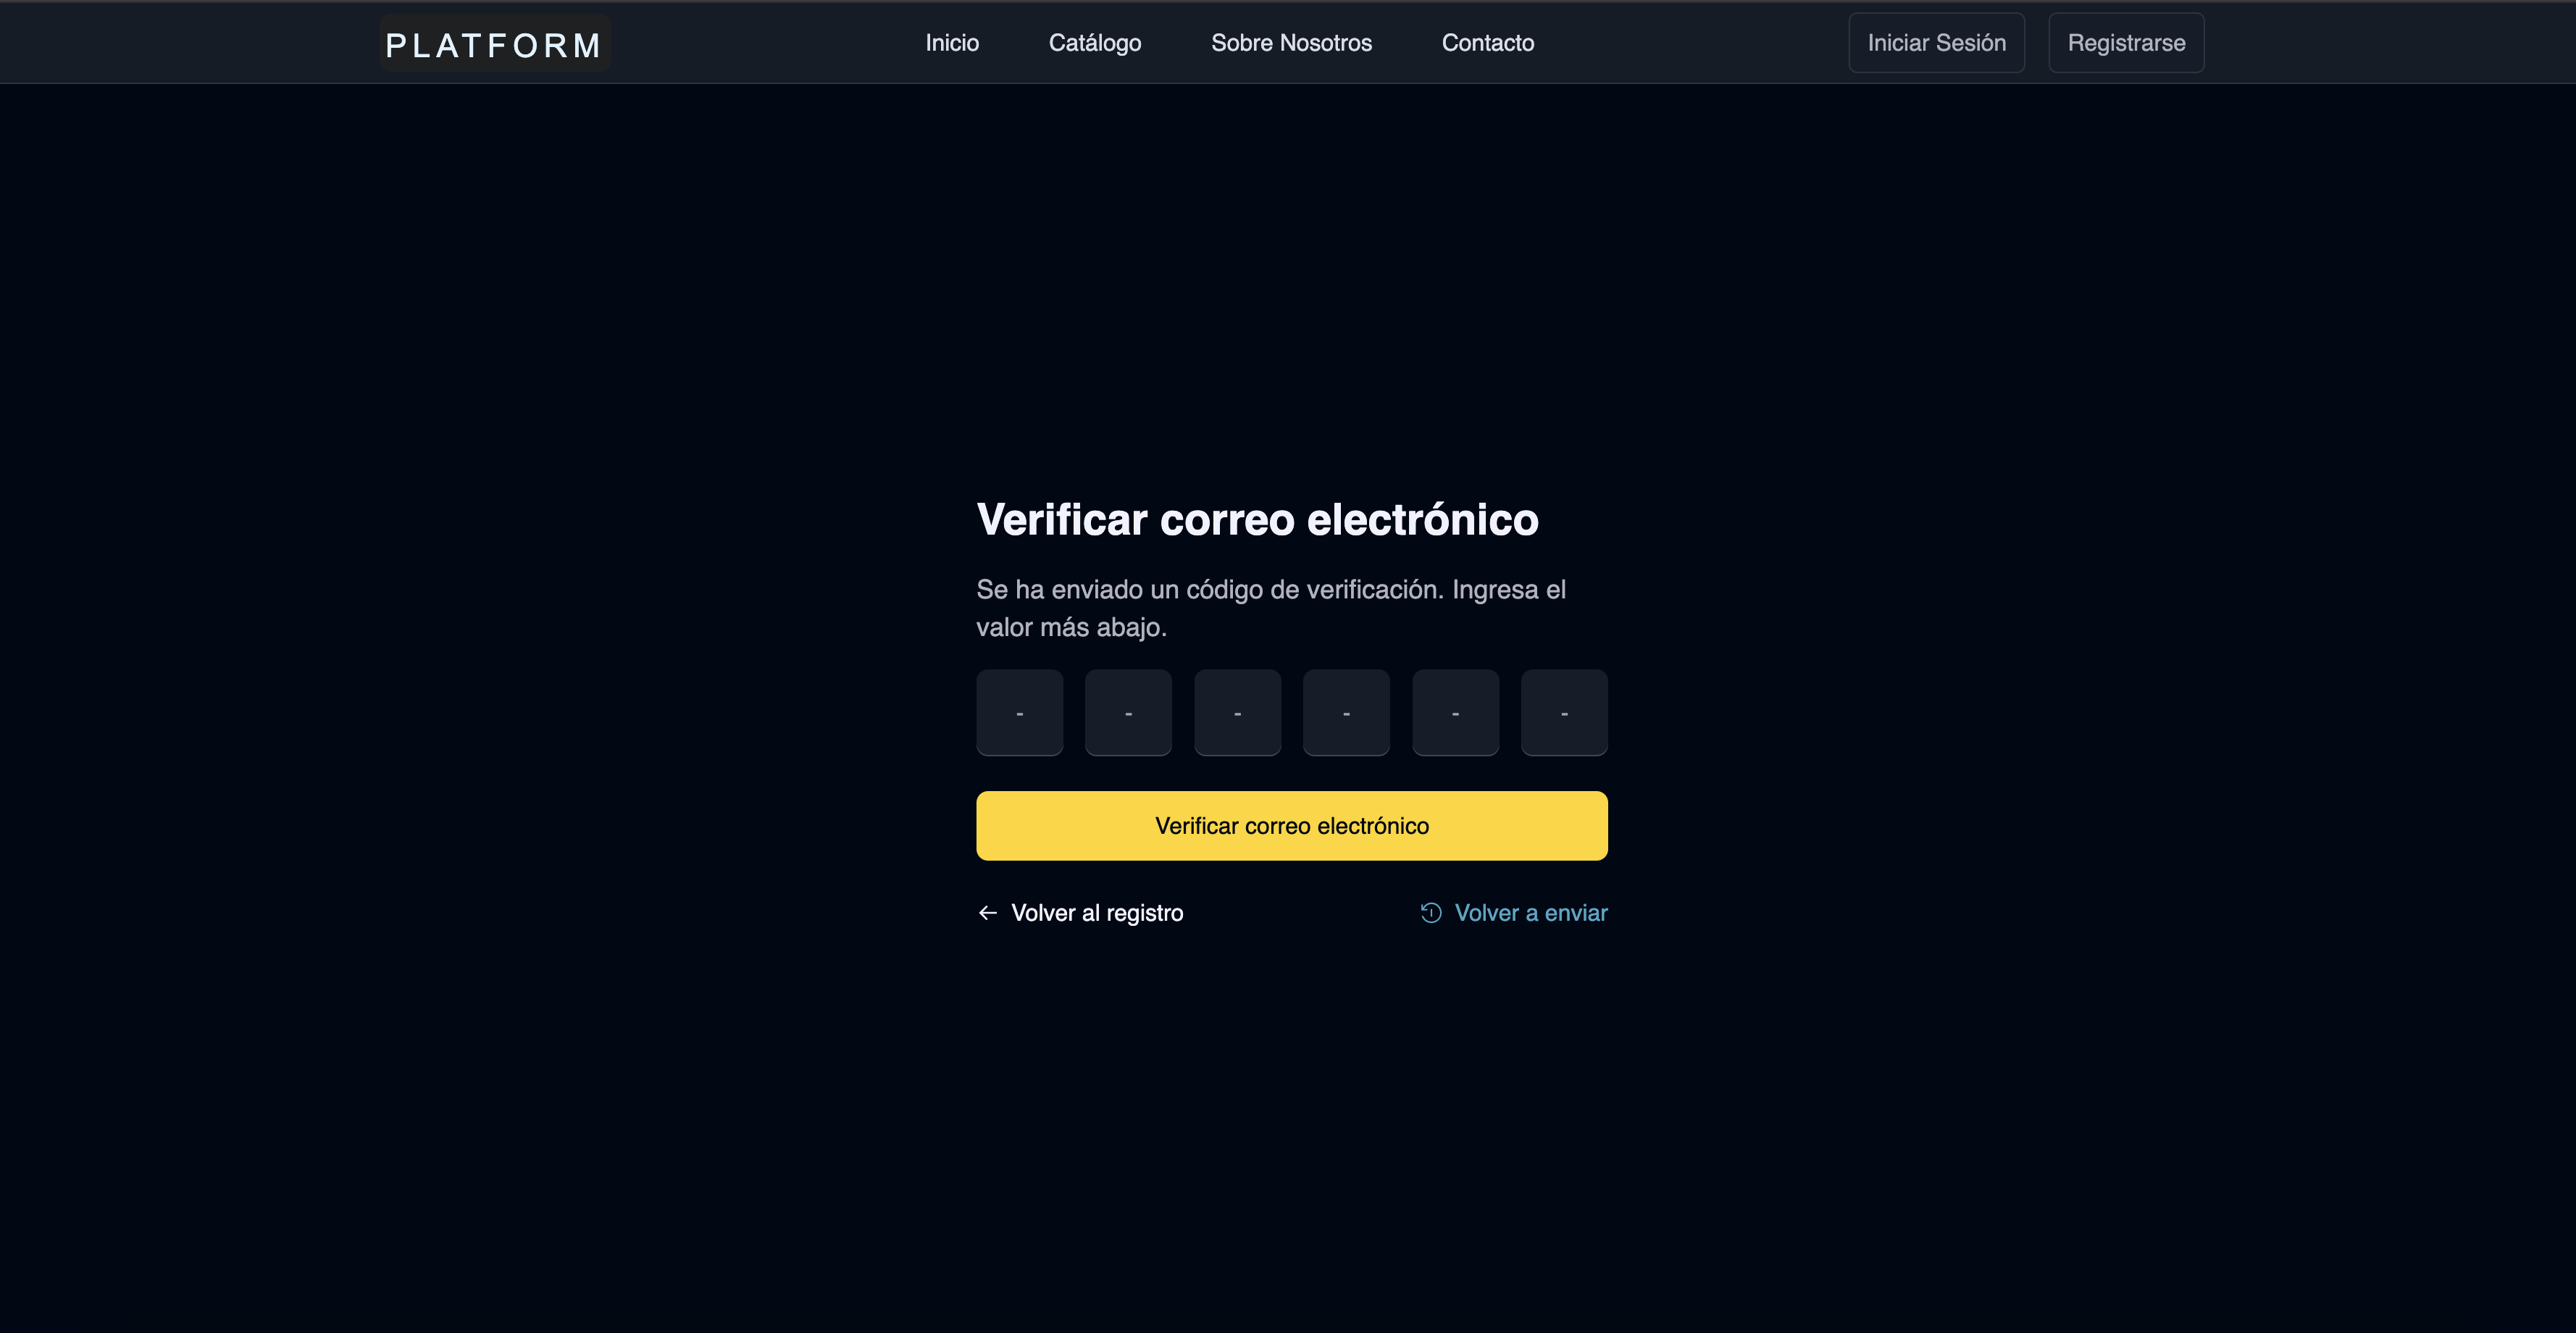
\includegraphics[width=\linewidth]{plataforma/plataforma_04.png}
    \caption{Interfaz de verificar correo}
    \label{fig:interfaz_sistema_verificar_correo}
\end{figure}

\begin{figure}[H]
    \centering
    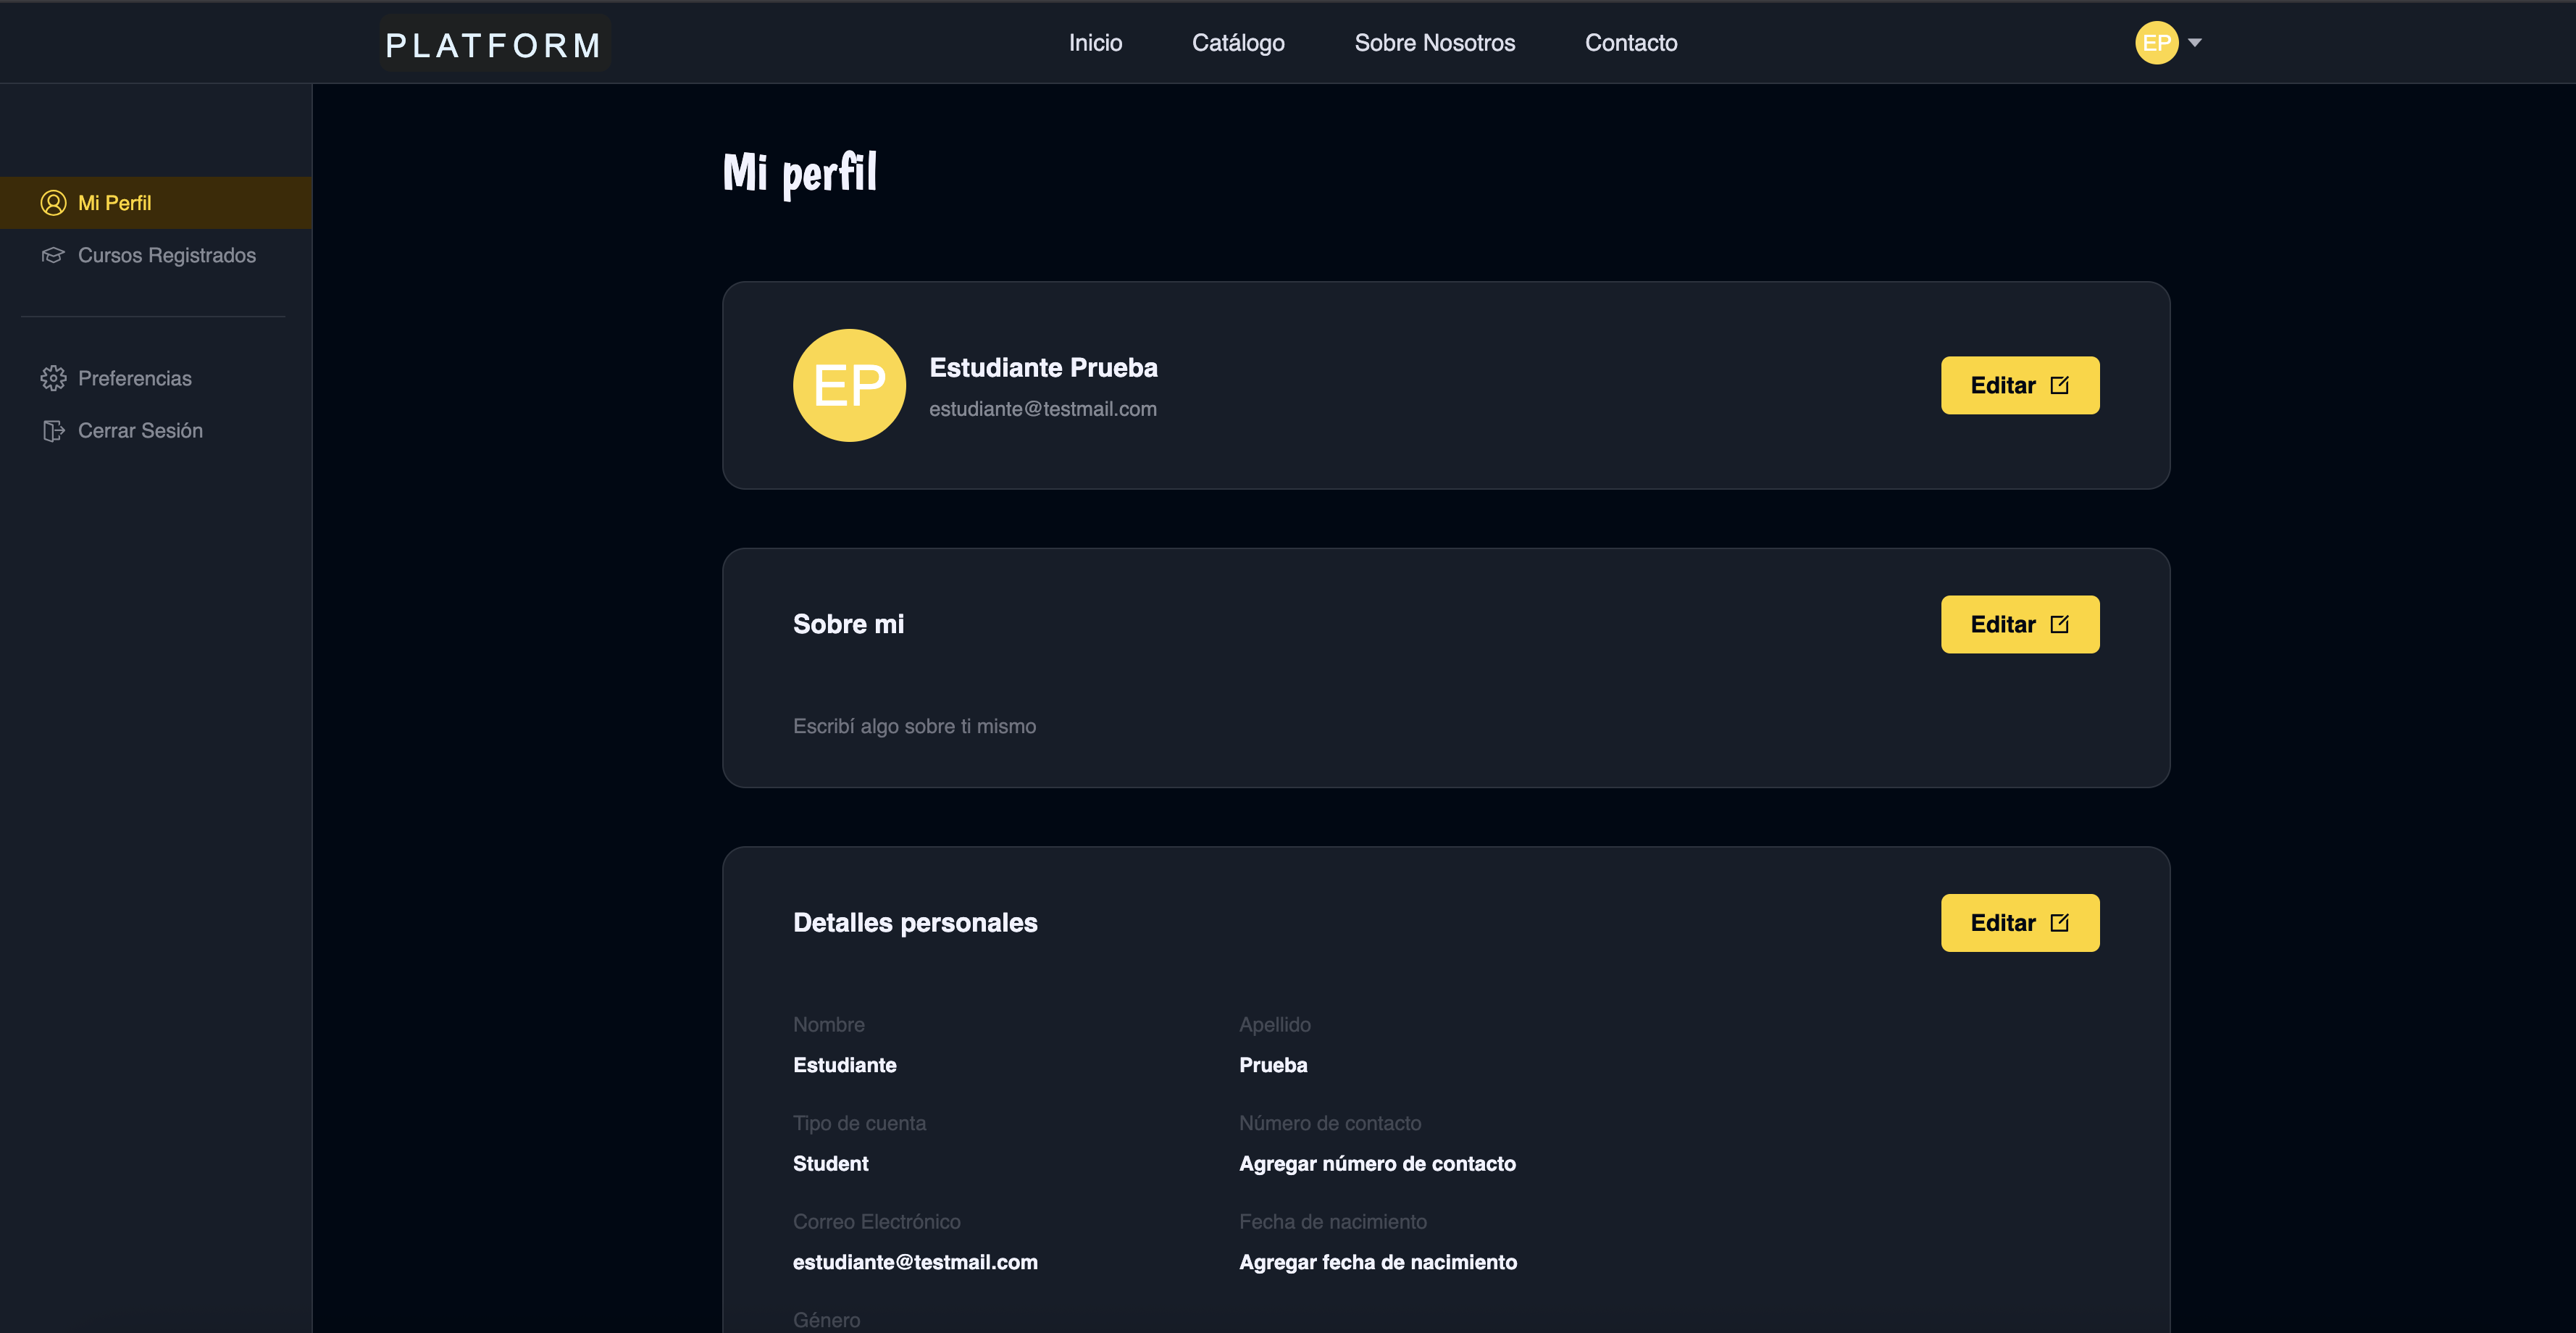
\includegraphics[width=\linewidth]{plataforma/plataforma_05.png}
    \caption{Interfaz de perfil de usuario}
    \label{fig:interfaz_sistema_perfil_usuario}
\end{figure}

\begin{figure}[H]
    \centering
    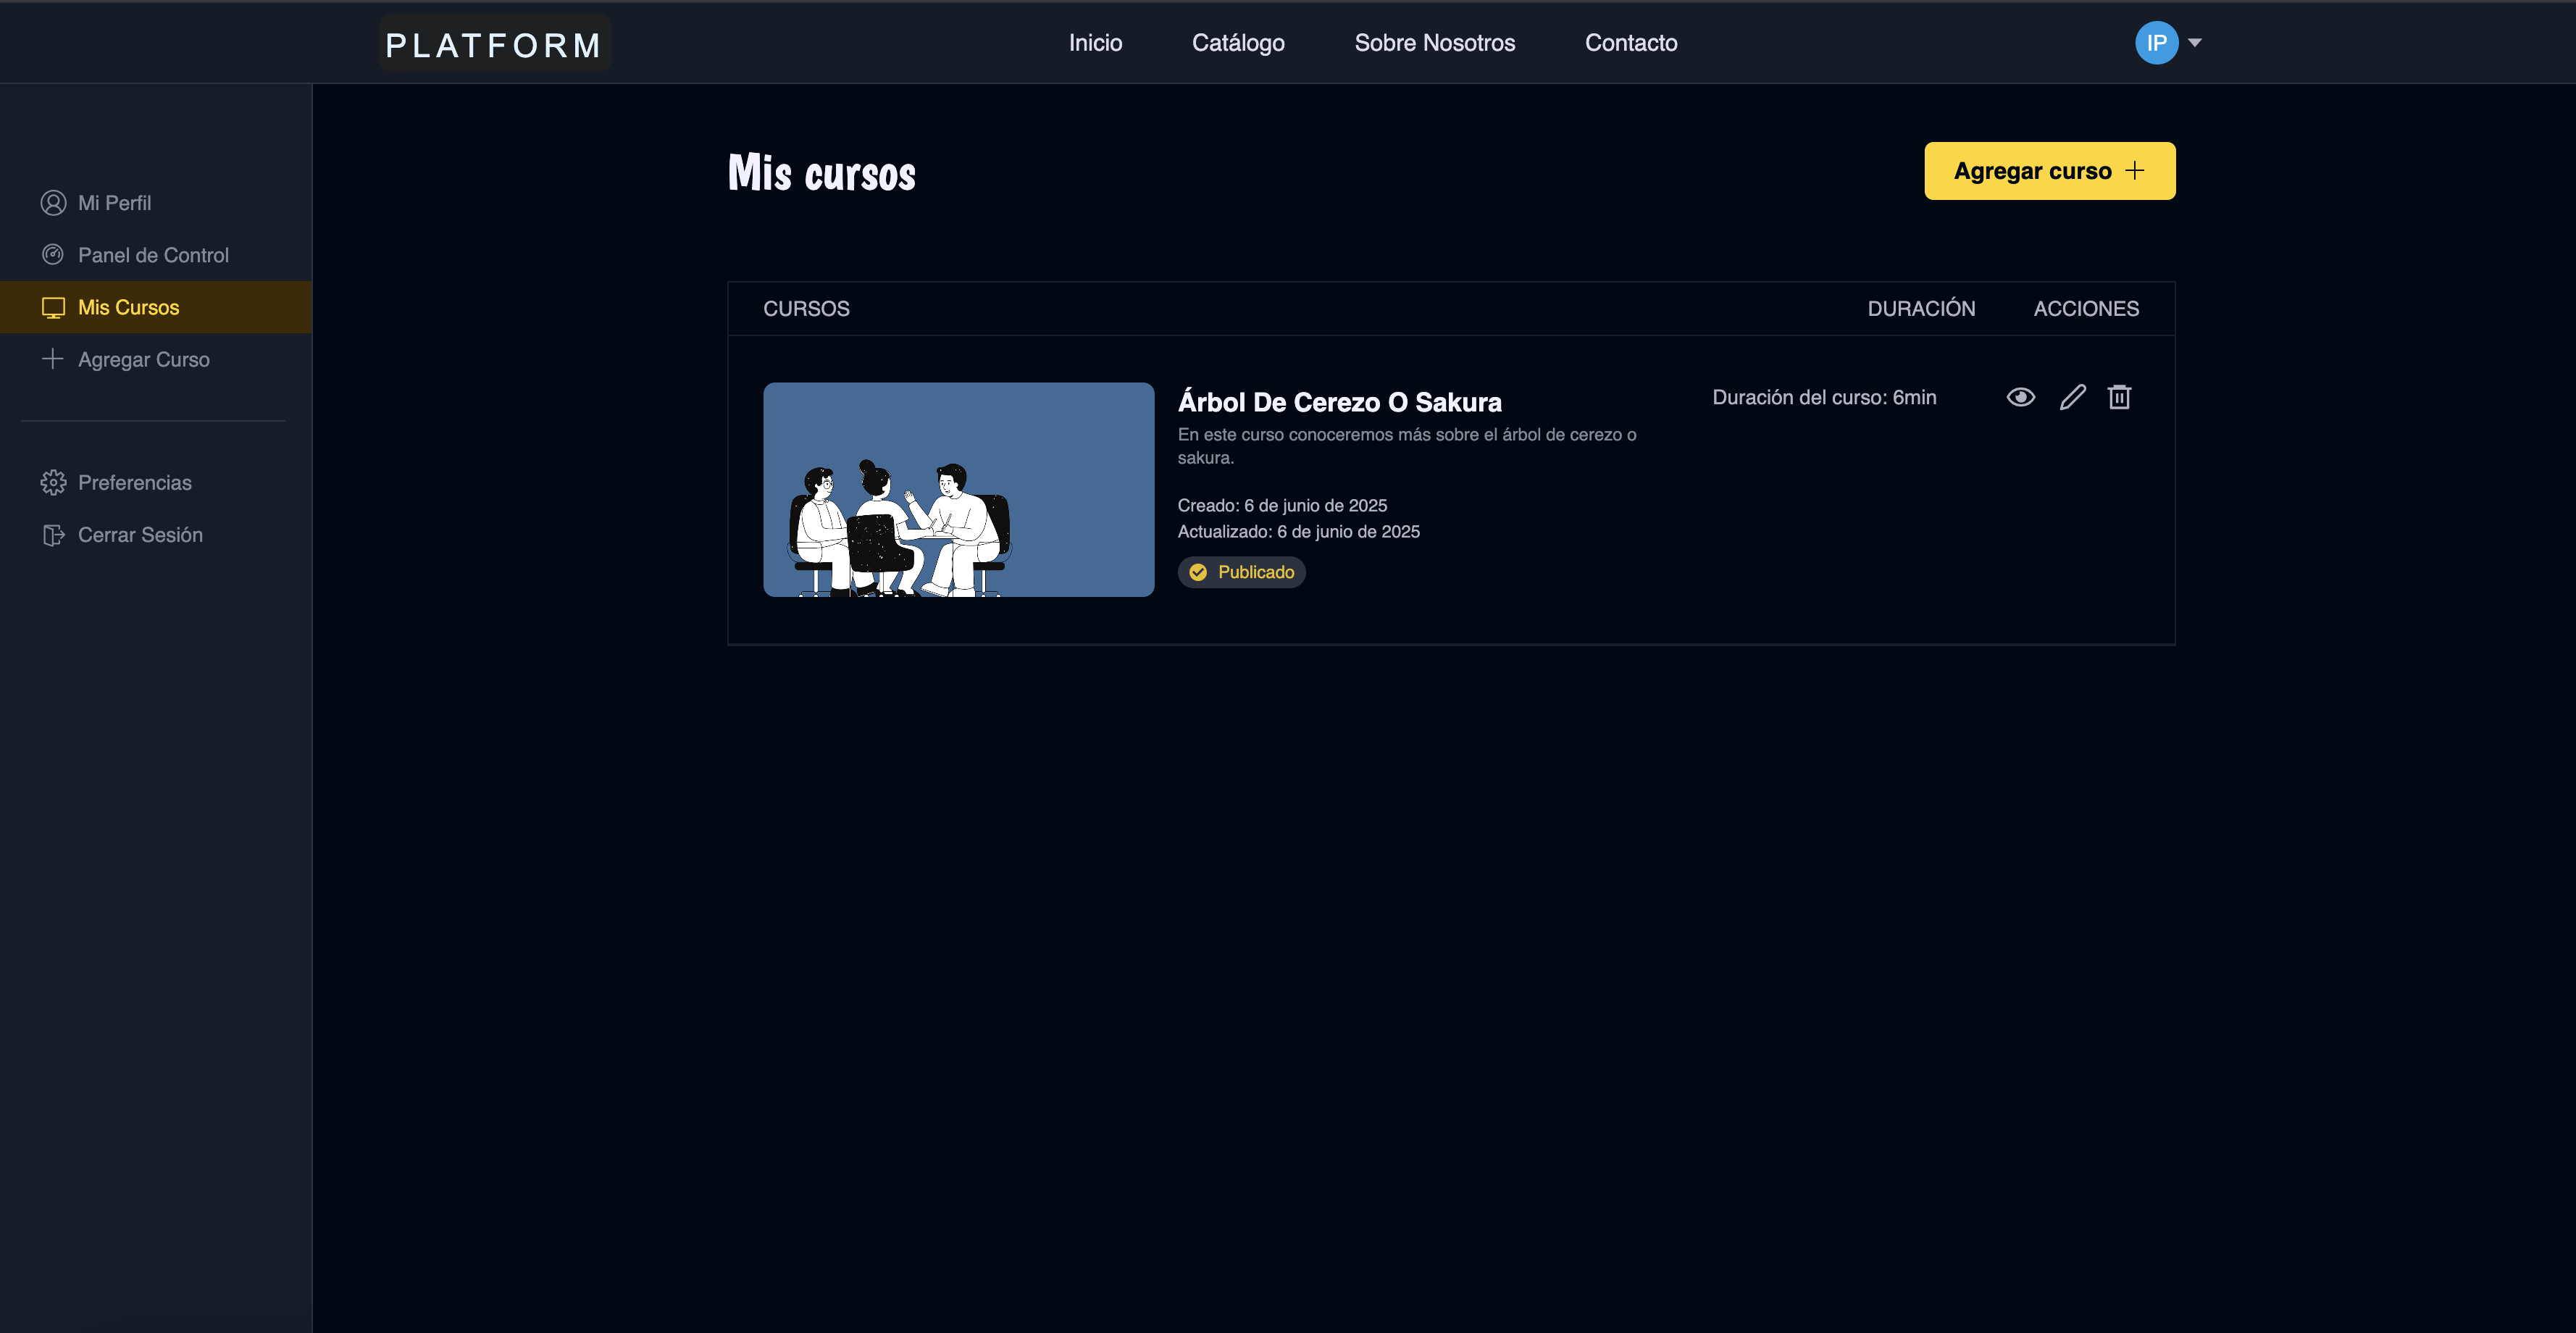
\includegraphics[width=\linewidth]{plataforma/plataforma_06.png}
    \caption{Interfaz de cursos del usuario instructor}
    \label{fig:interfaz_sistema_cursos_usuario_instructor}
\end{figure}

\begin{figure}[H]
    \centering
    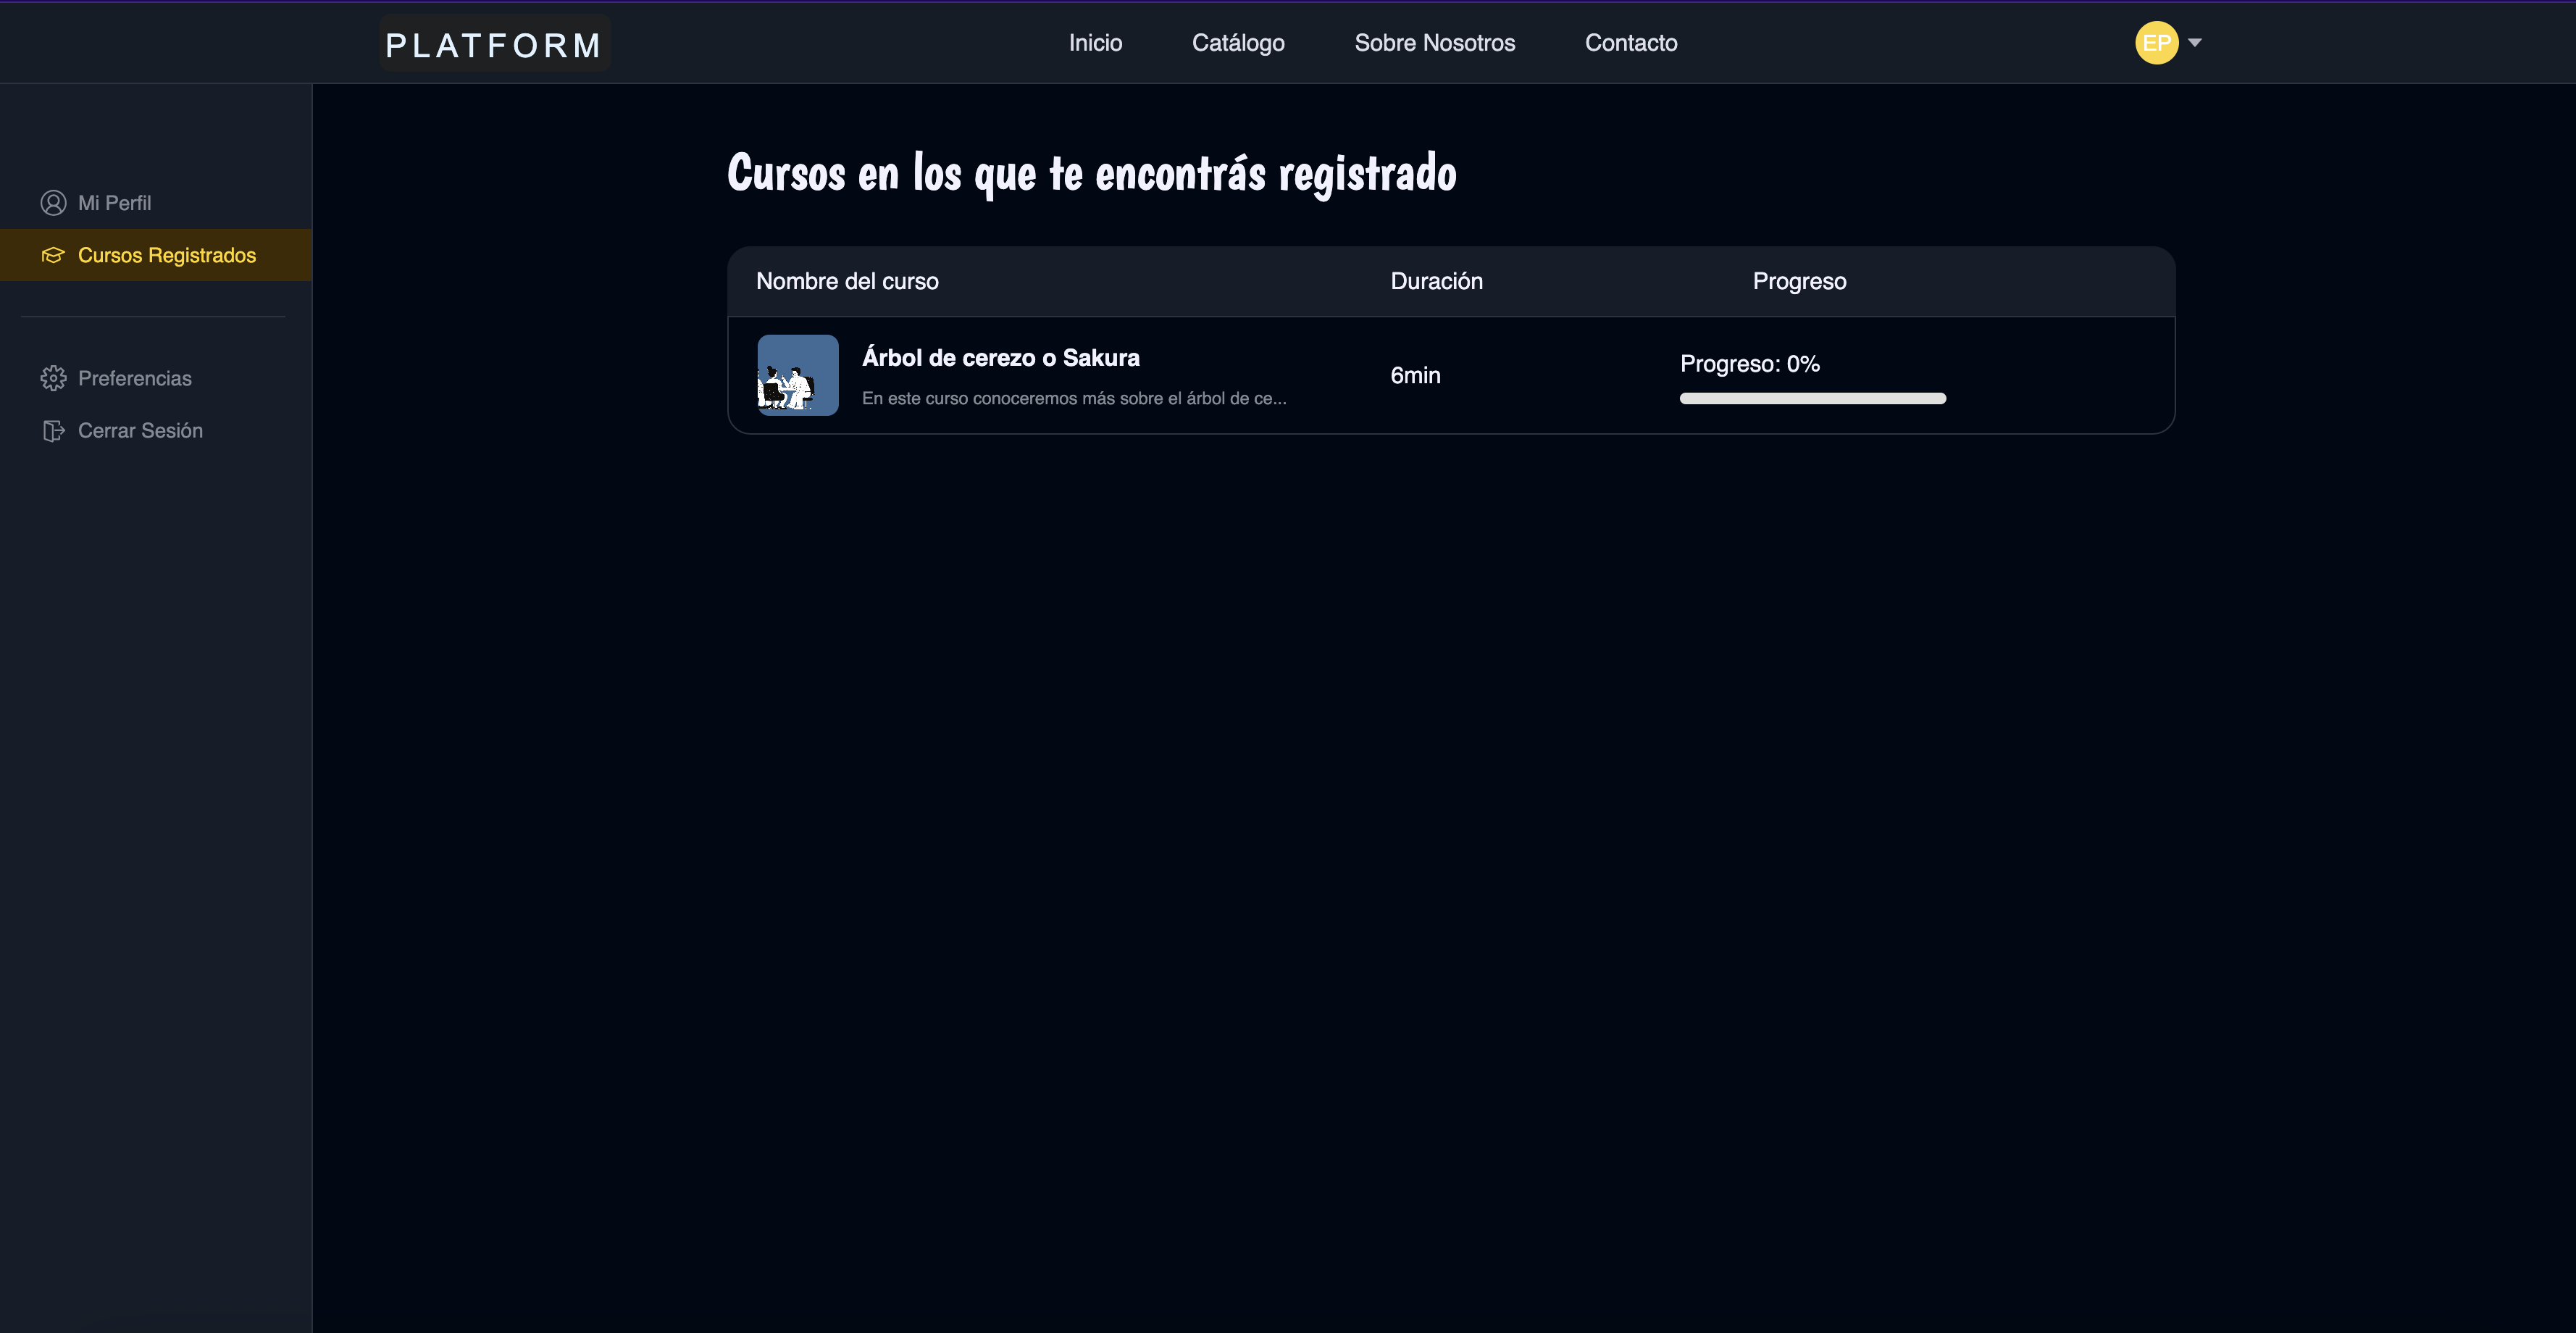
\includegraphics[width=\linewidth]{plataforma/plataforma_08.png}
    \caption{Interfaz de cursos del usuario estudiante}
    \label{fig:interfaz_sistema_cursos_usuario_estudiante}
\end{figure}


\section{Lecciones en Imágenes}

\begin{figure}[H]
    \centering
    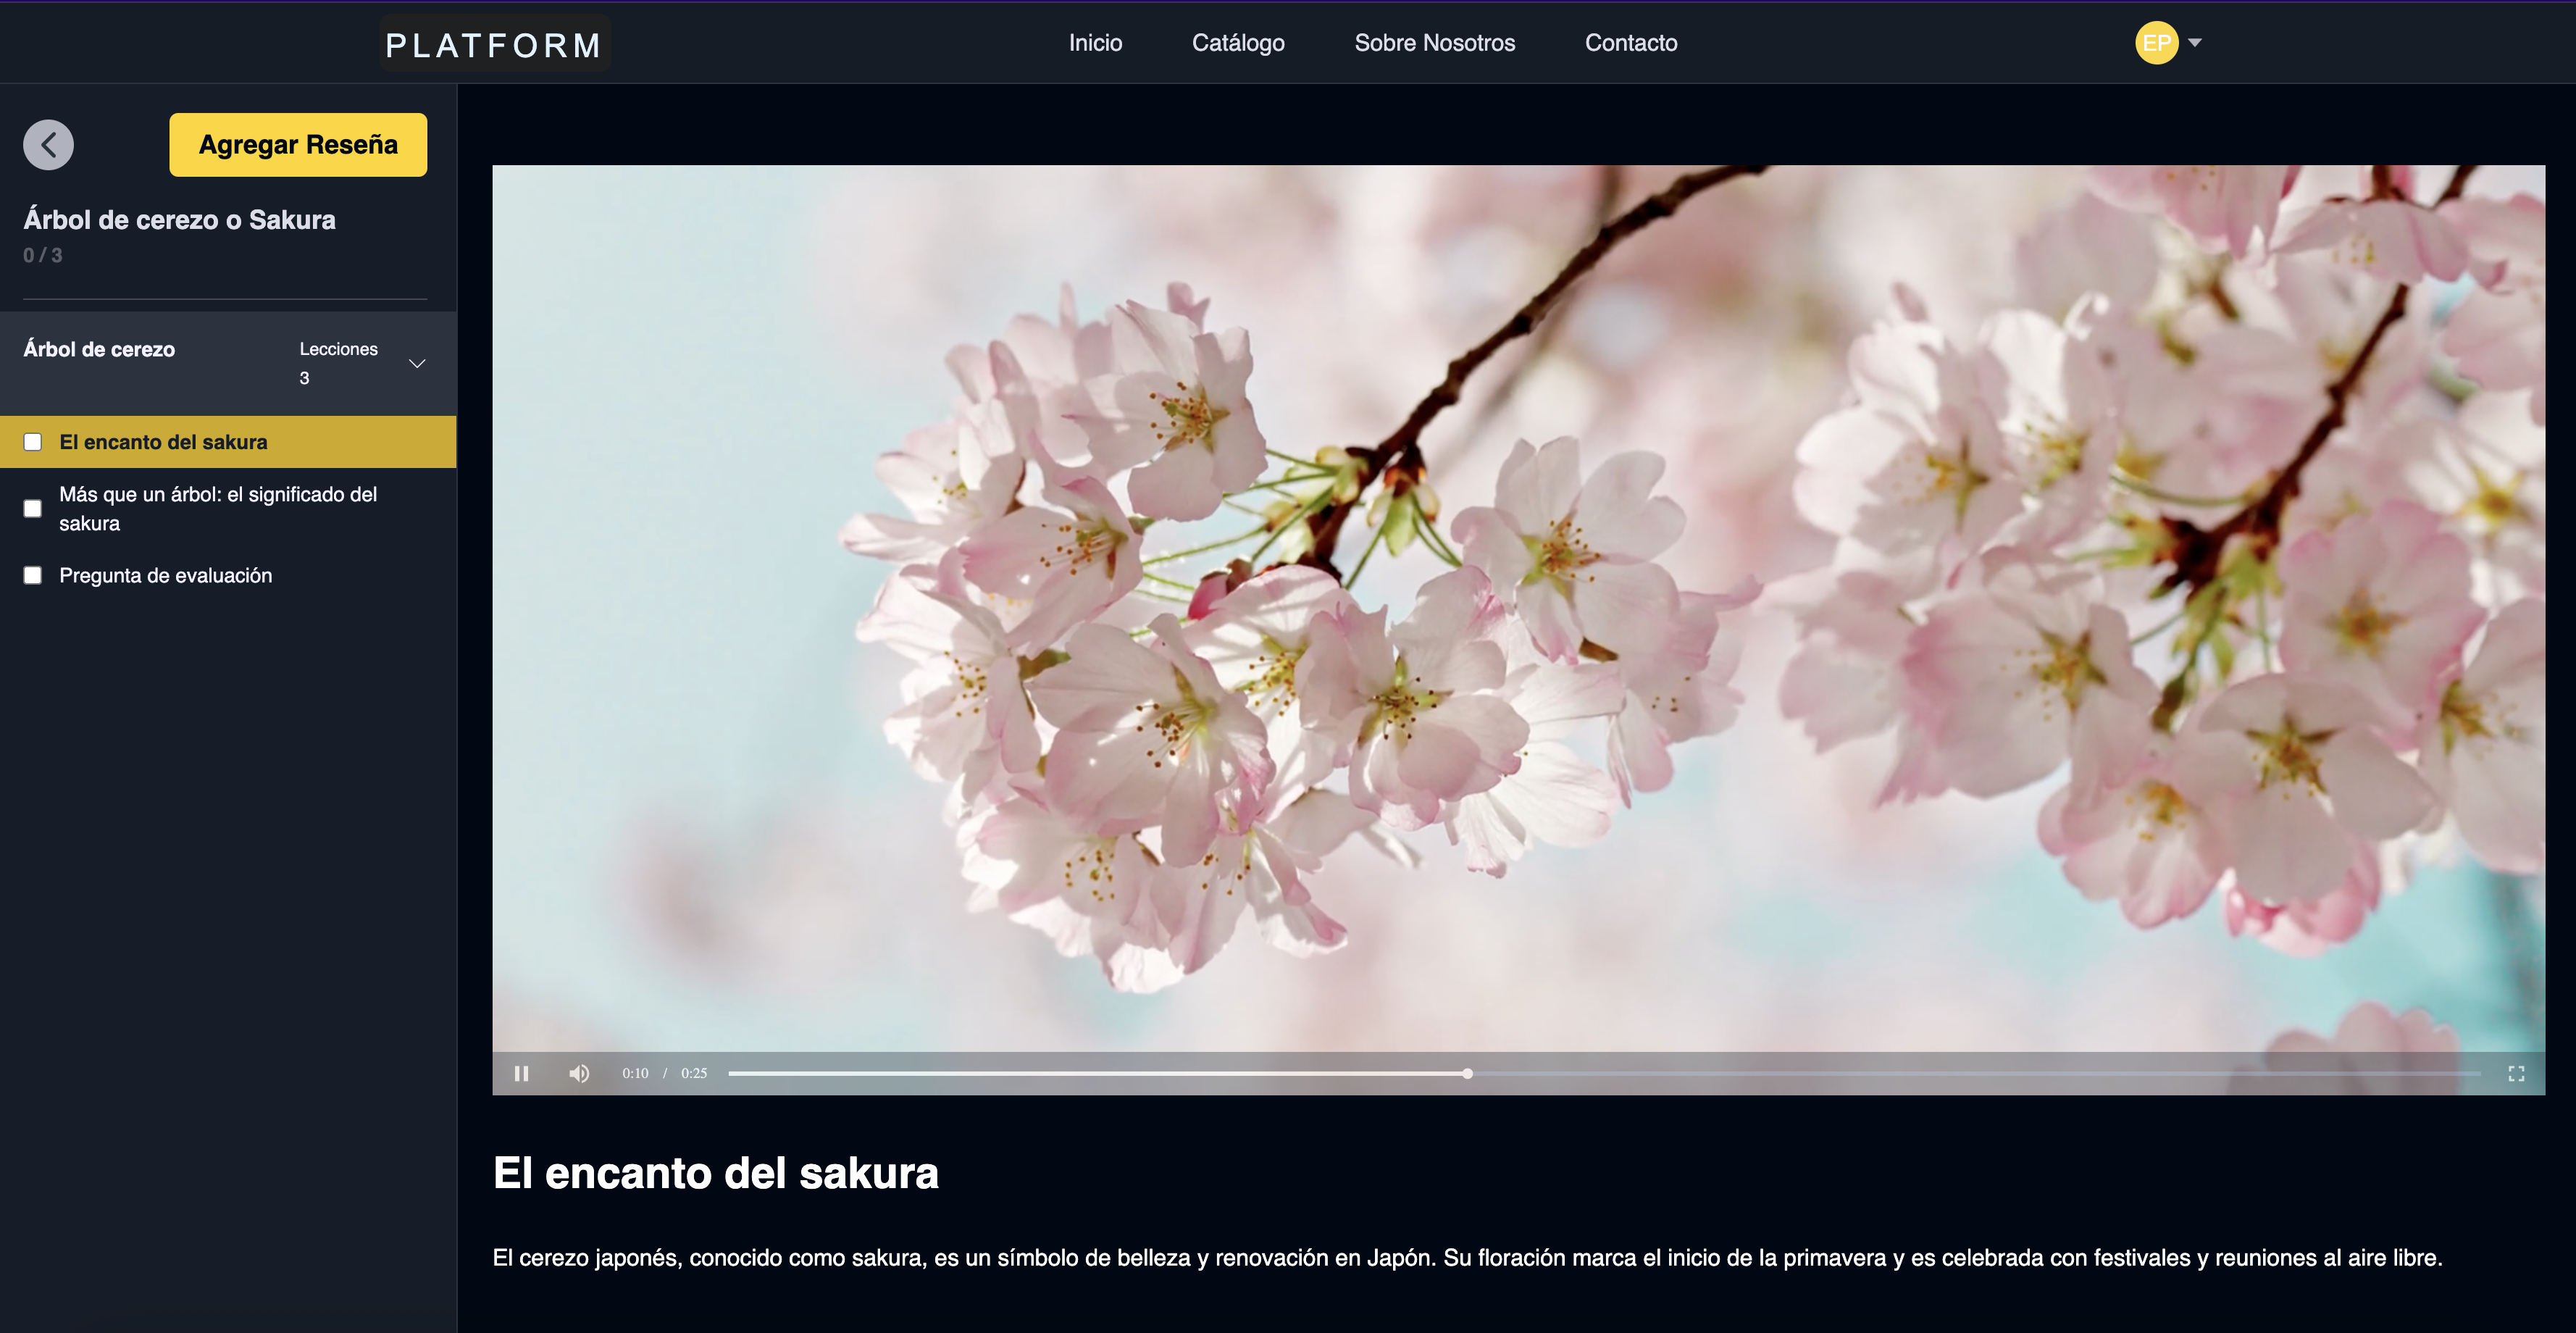
\includegraphics[width=\linewidth]{leccion/leccion_01.png}
    \caption{Lección de video}
    \label{fig:leccion_video}
\end{figure}

\begin{figure}[H]
    \centering
    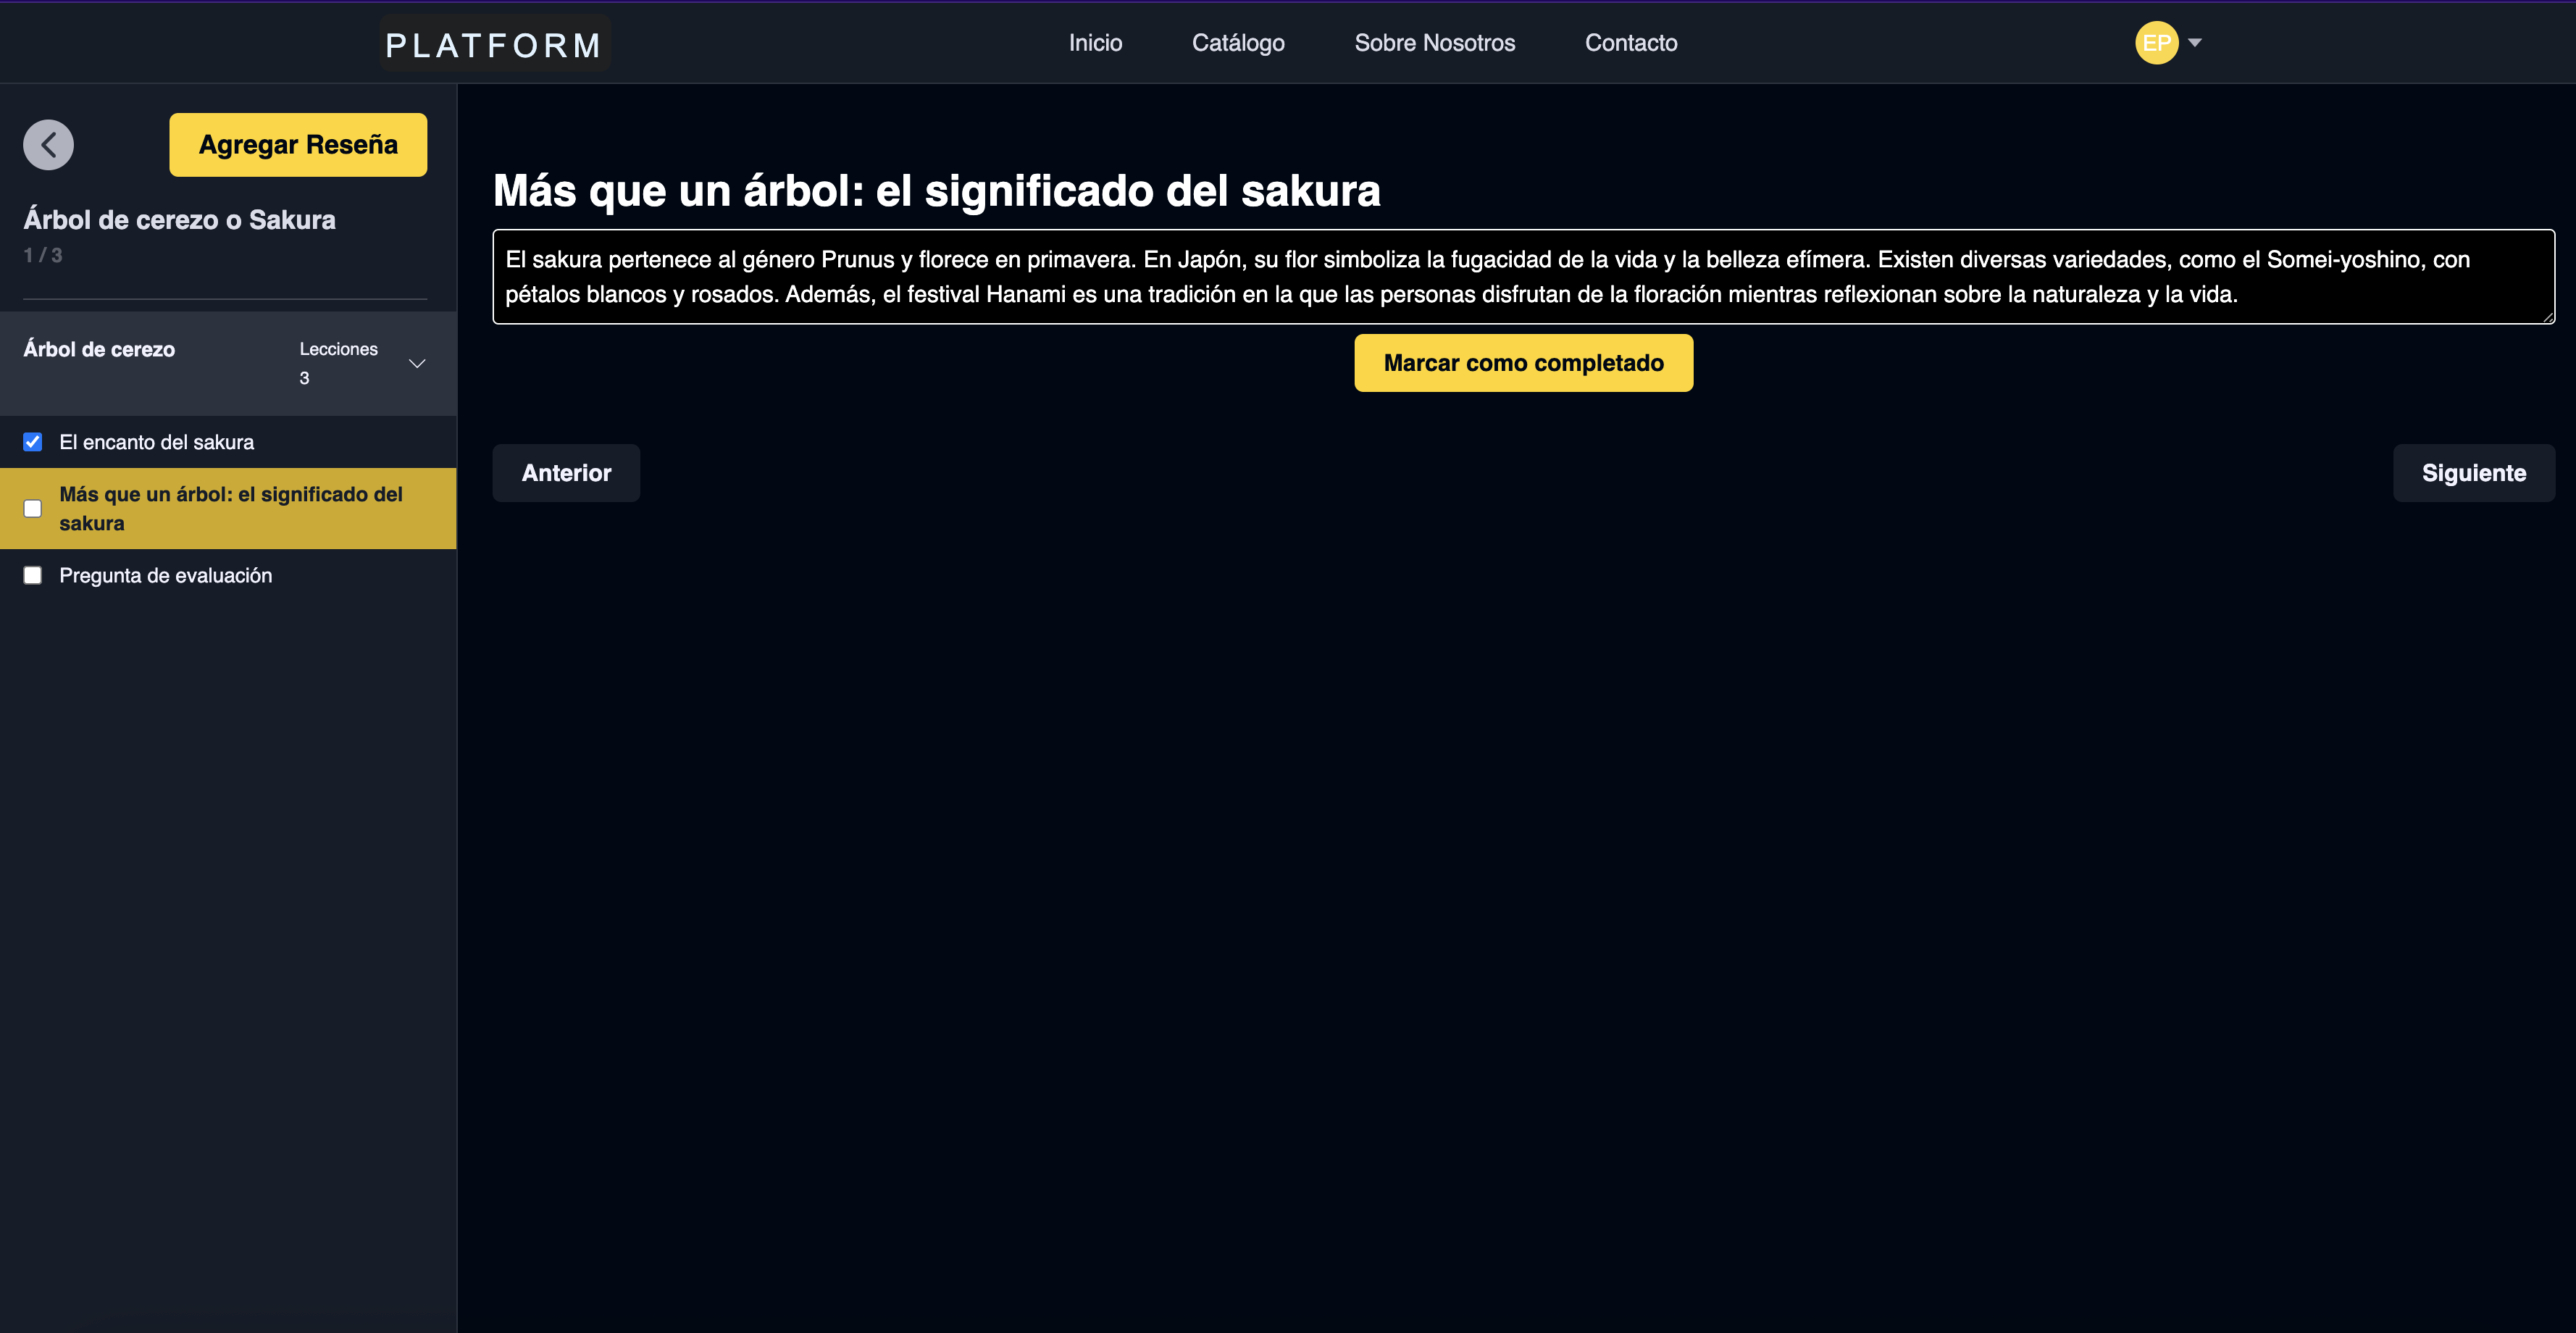
\includegraphics[width=\linewidth]{leccion/leccion_02.png}
    \caption{Lección de texto}
    \label{fig:leccion_texto}
\end{figure}

\begin{figure}[H]
    \centering
    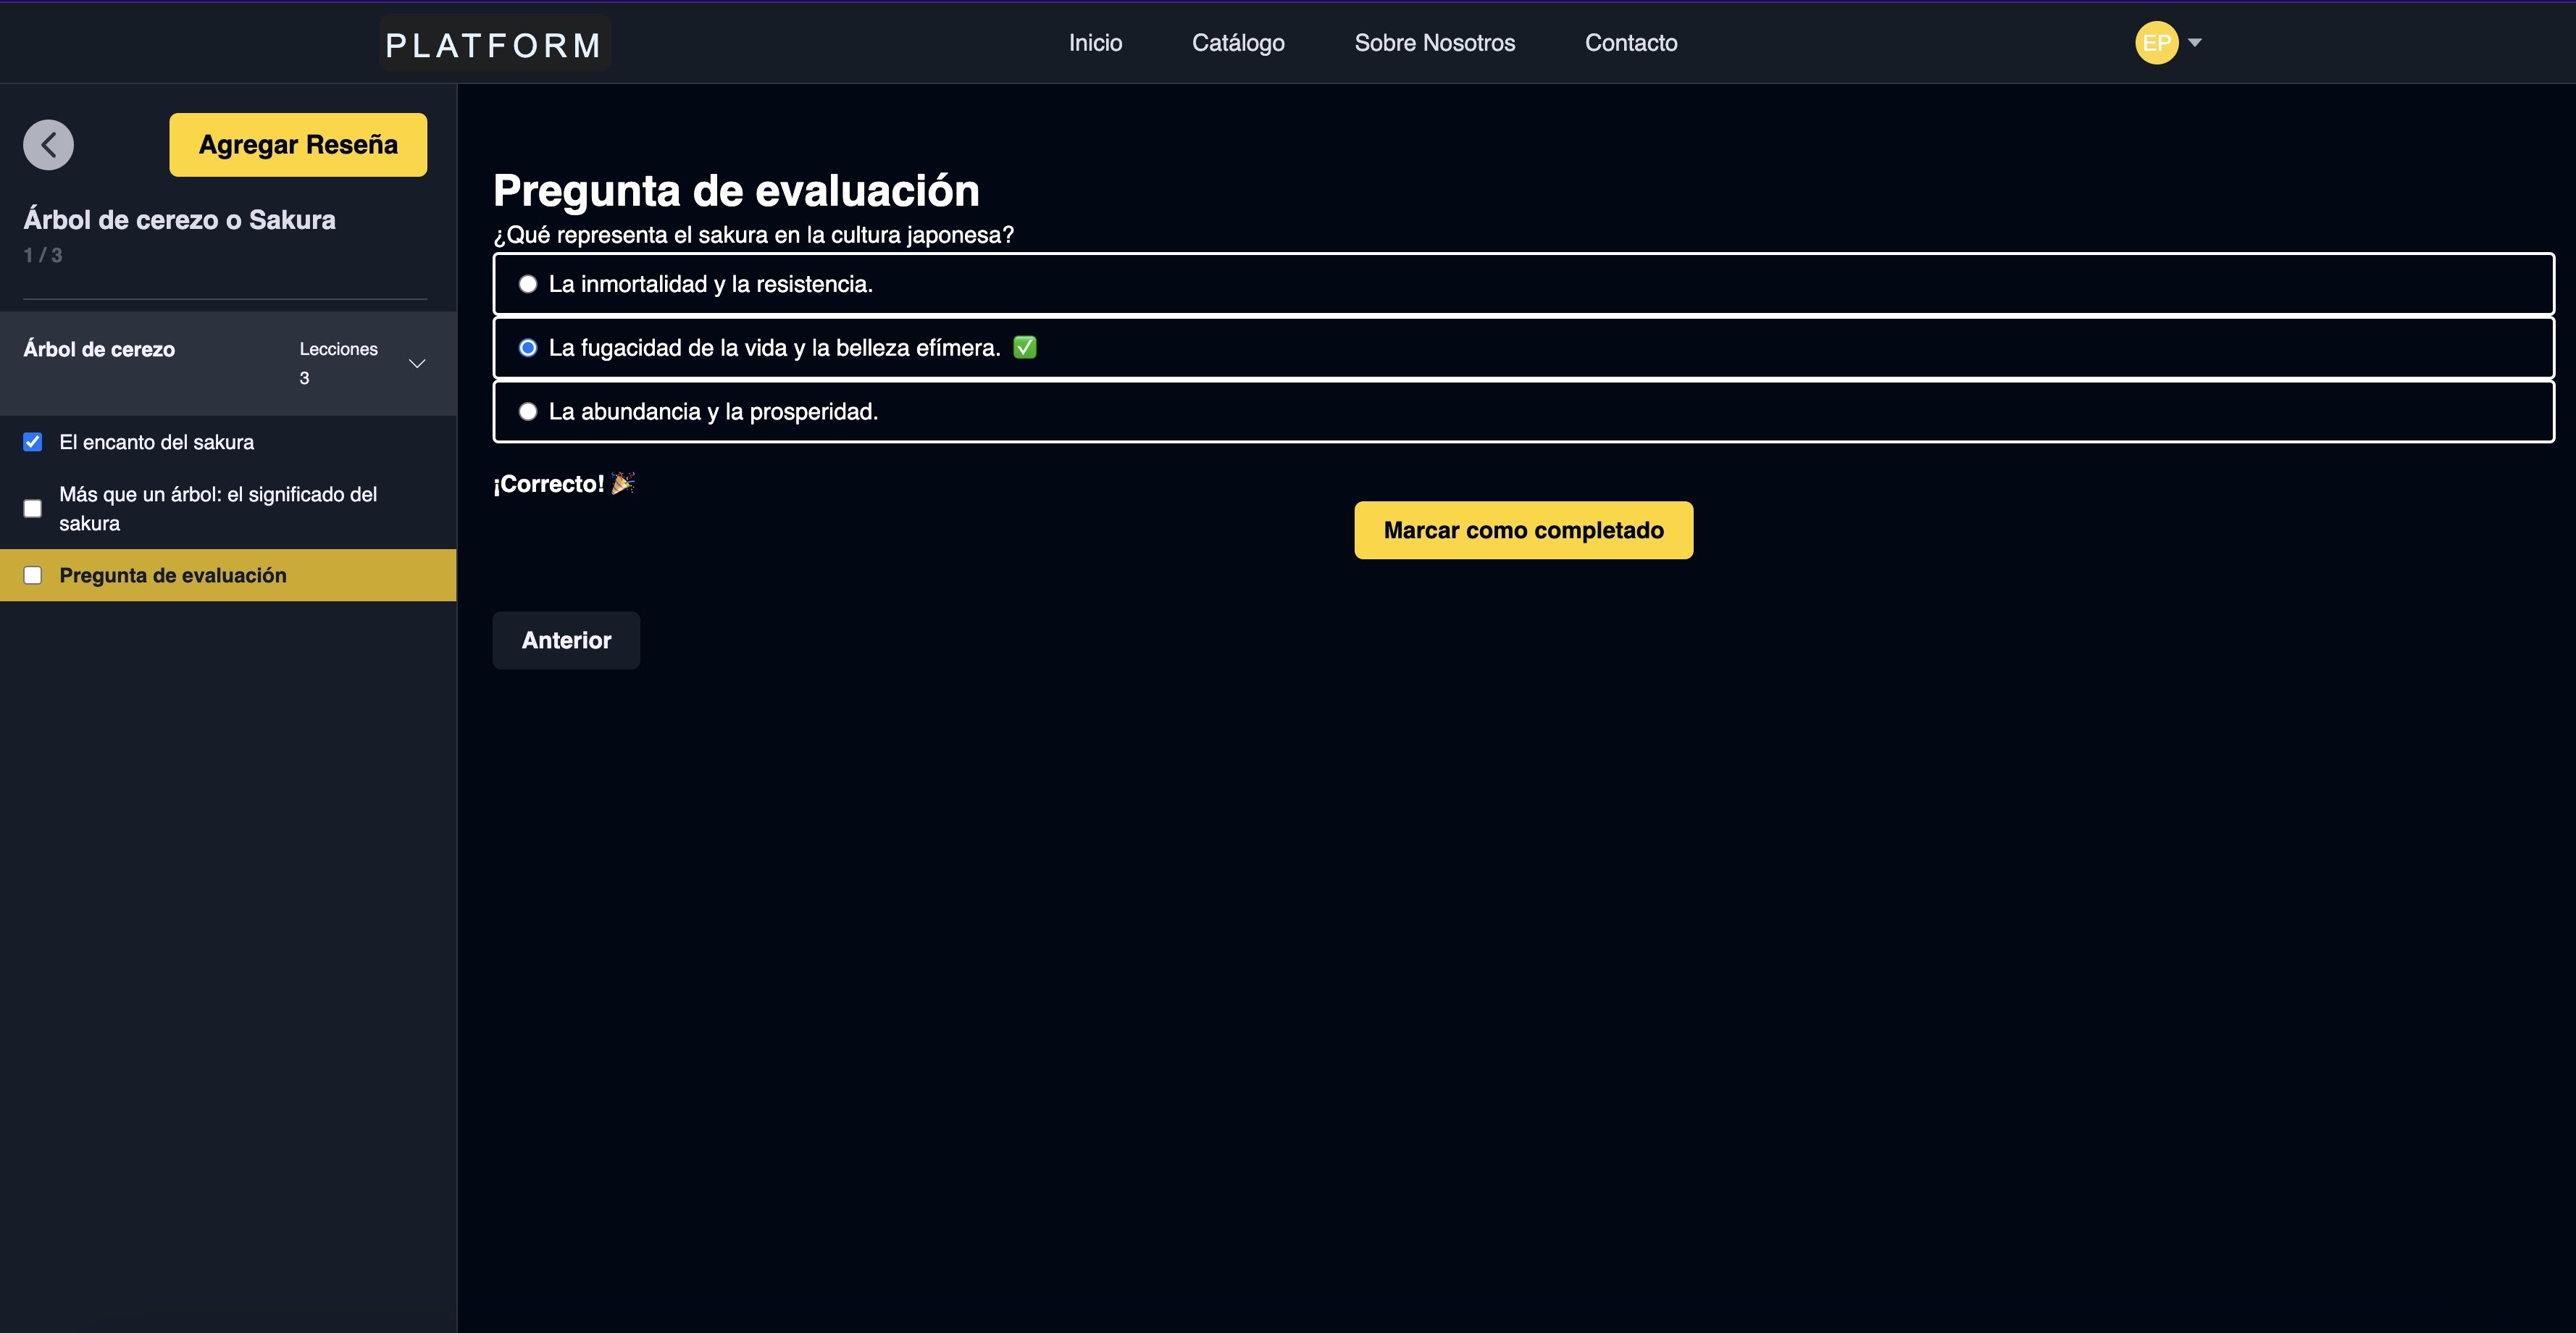
\includegraphics[width=\linewidth]{leccion/leccion_03.png}
    \caption{Lección de opción mútiple}
    \label{fig:leccion_opcion_multiple}
\end{figure}

\section{Integración con Telegram en Imágenes}

\begin{figure}[H]
    \centering
    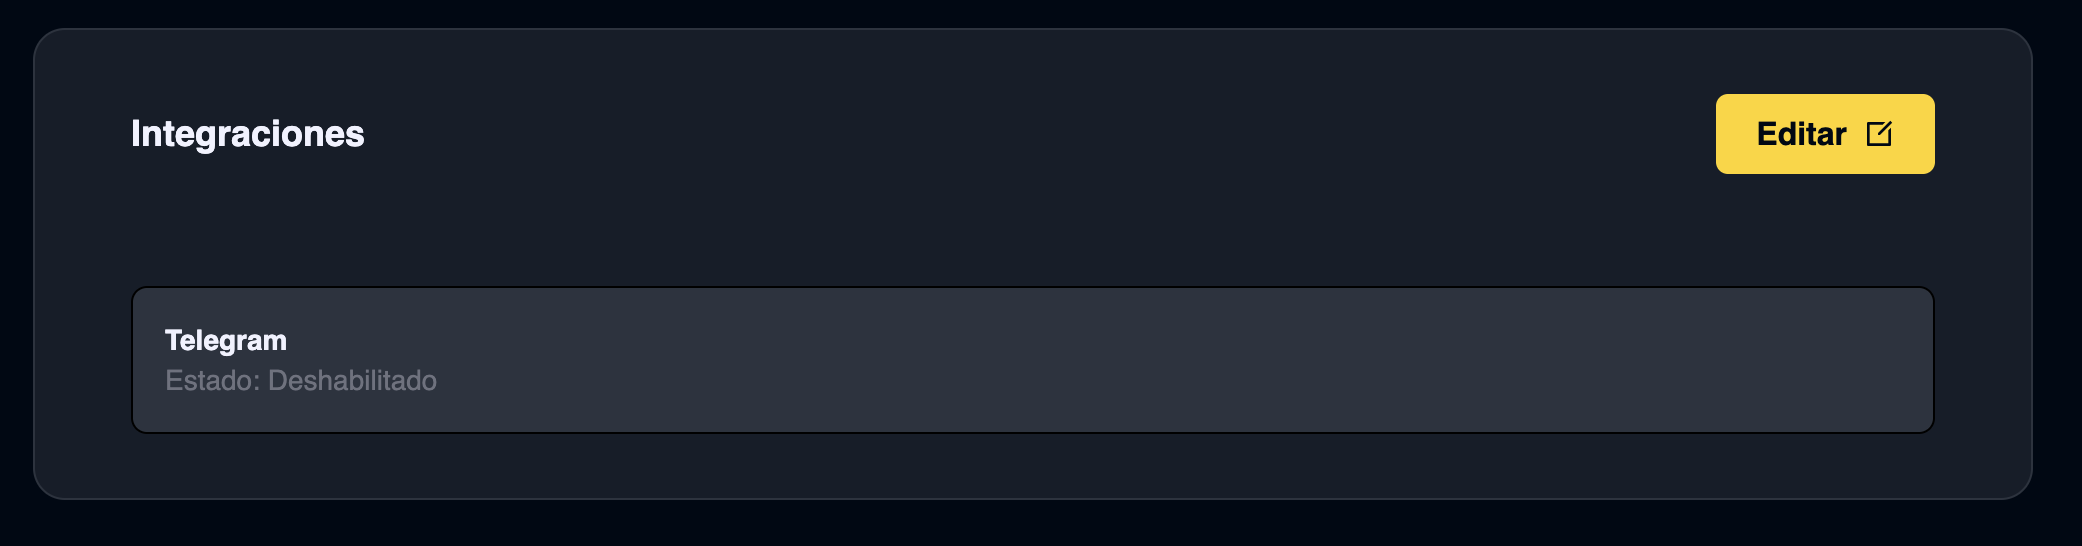
\includegraphics[width=\linewidth]{integracion_telegram/integracion_telegram_01.png}
    \caption{Integración deshabilitada}
    \label{fig:integracion_telegram_deshabilitada}
\end{figure}

\begin{figure}[H]
    \centering
    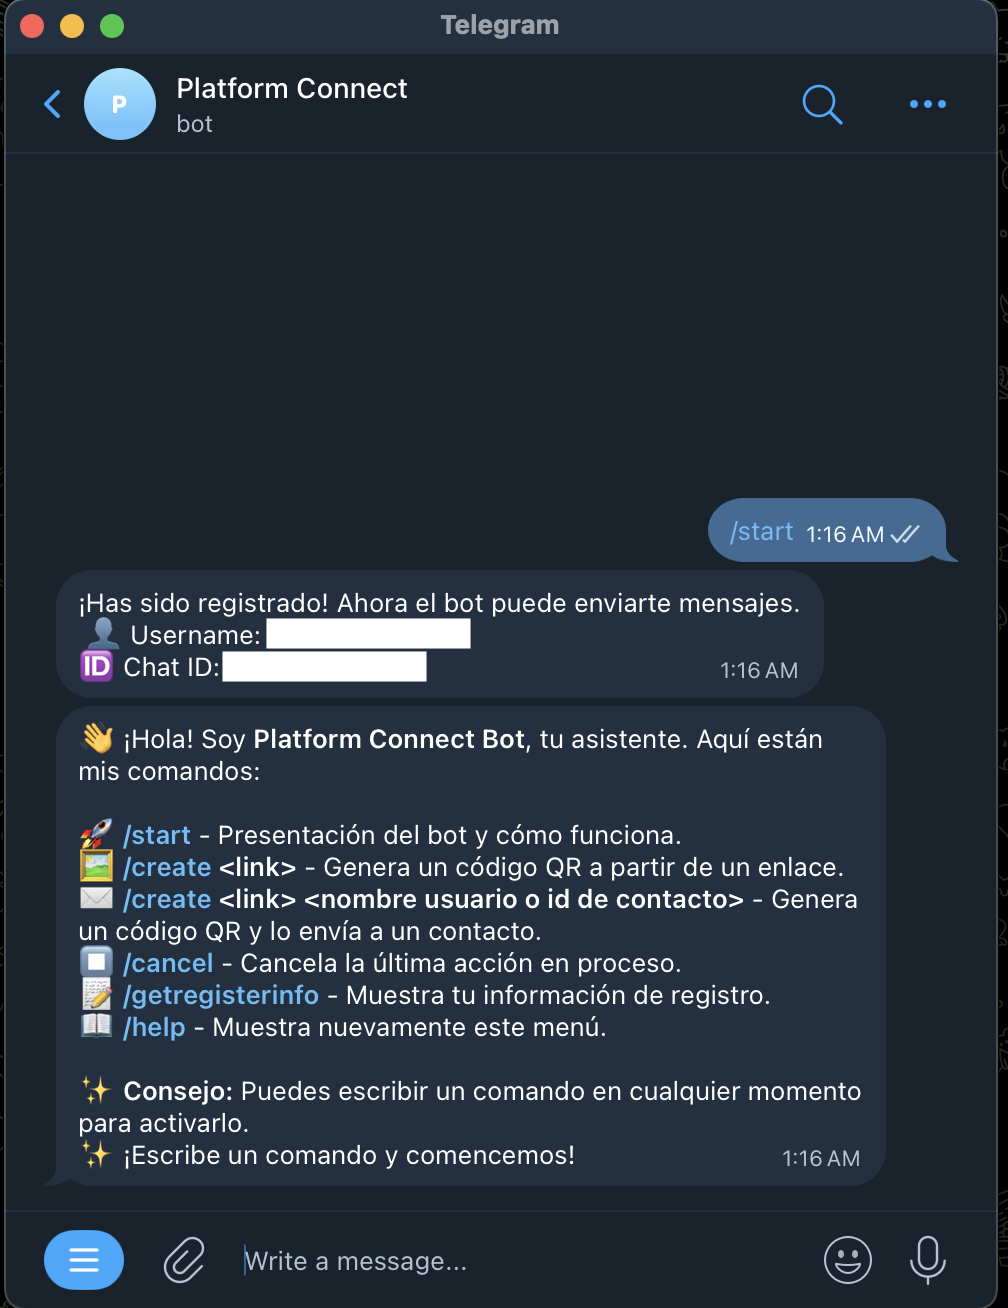
\includegraphics[width=\linewidth]{integracion_telegram/integracion_telegram_03.png}
    \caption{Registro de usuario en el bot}
    \label{fig:integracion_telegram_registro_bot}
\end{figure}

\begin{figure}[H]
    \centering
    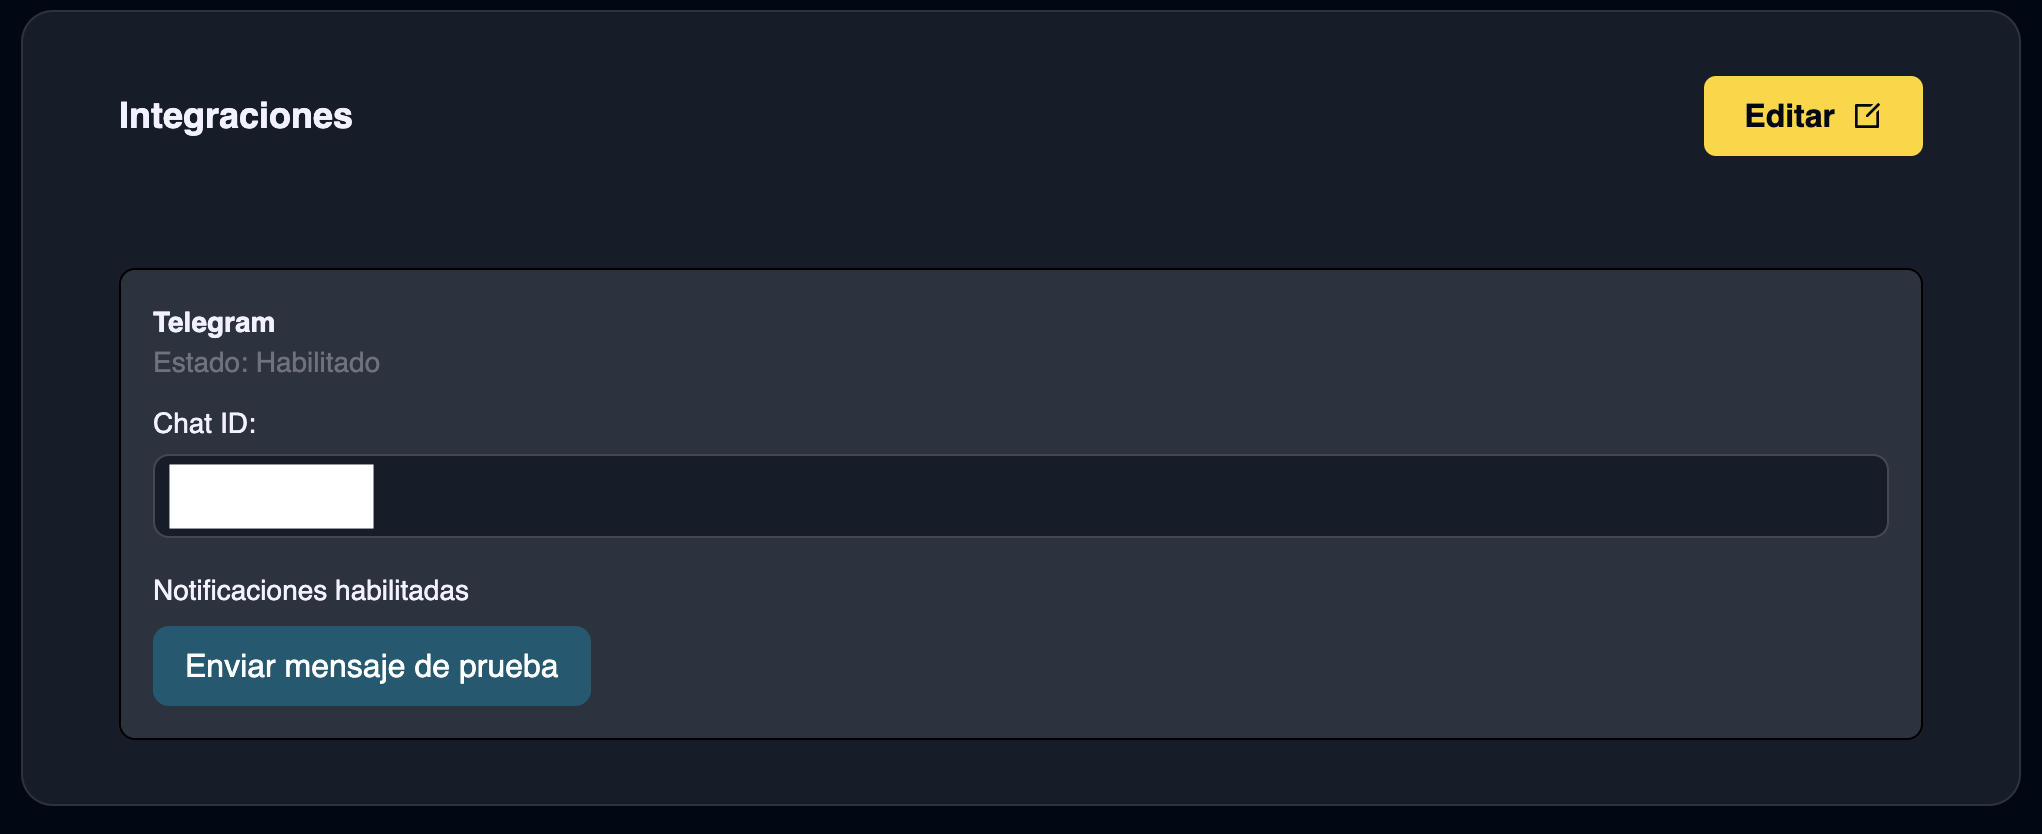
\includegraphics[width=\linewidth]{integracion_telegram/integracion_telegram_04.png}
    \caption{Integración habilitada}
    \label{fig:integracion_telegram_habilitada}
\end{figure}

\section{Integración con Sistema de Correos Electrónicos en Imágenes}

\begin{figure}[H]
    \centering
    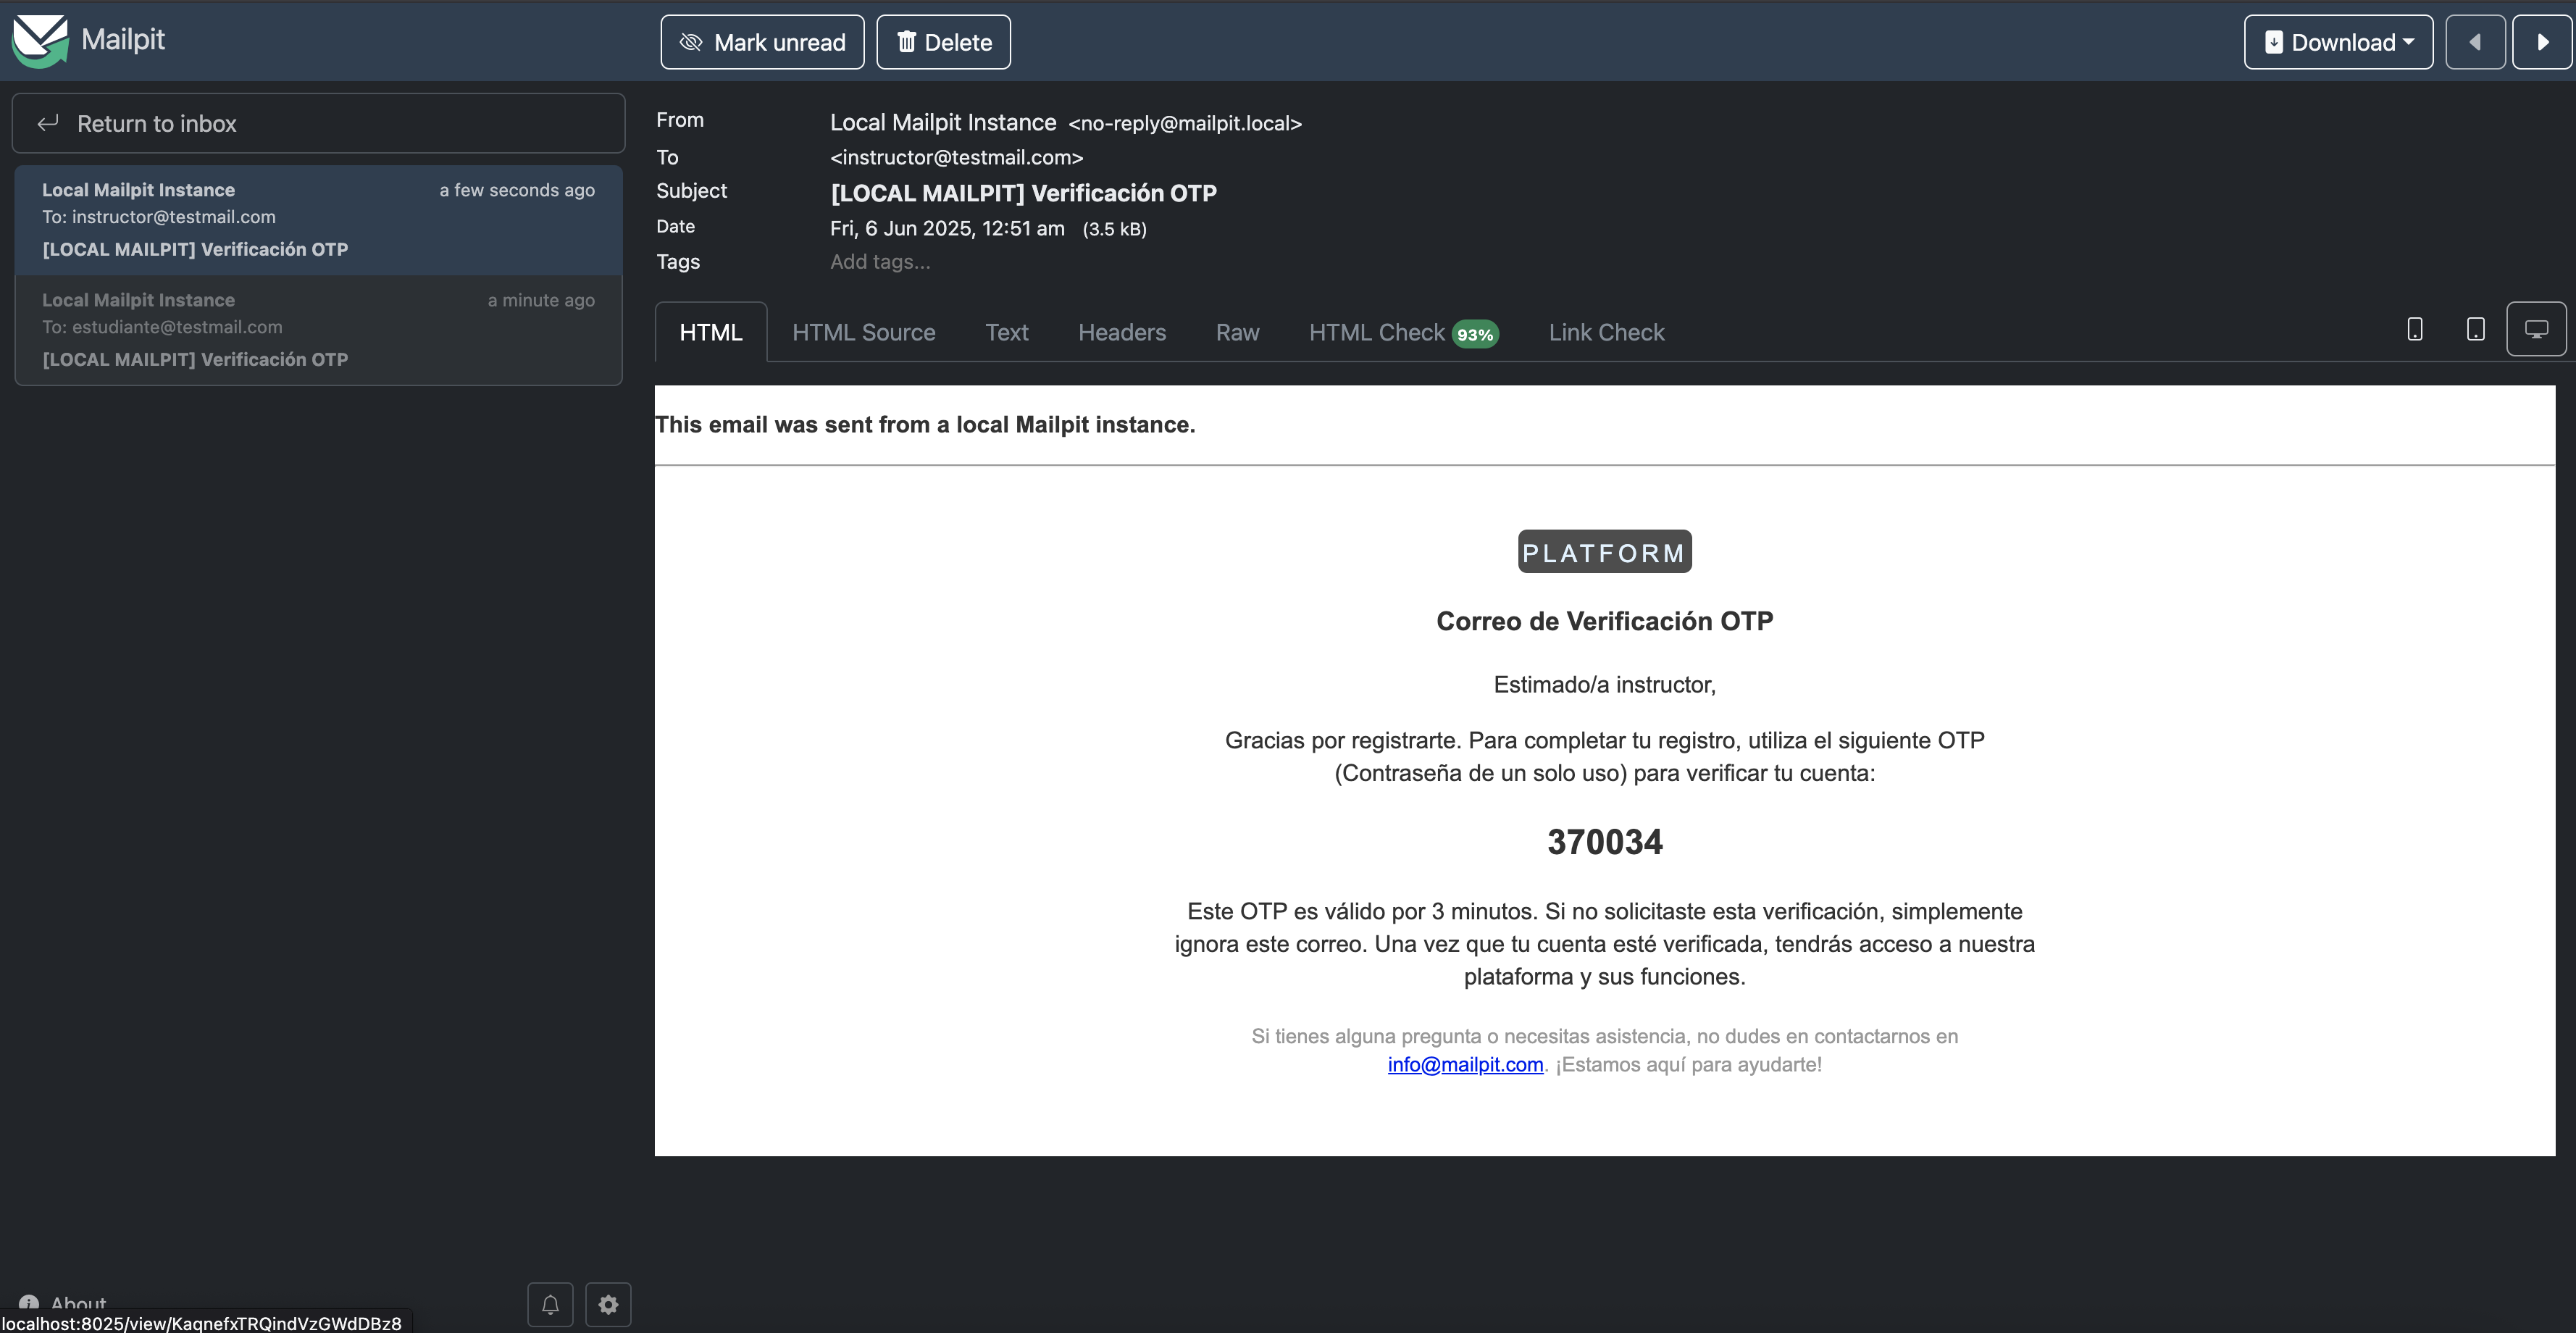
\includegraphics[width=\linewidth]{mail/mail_01.png}
    \caption{Correo de OTP}
    \label{fig:correo_electronico_otp}
\end{figure}
\begin{figure}[H]
    \centering
    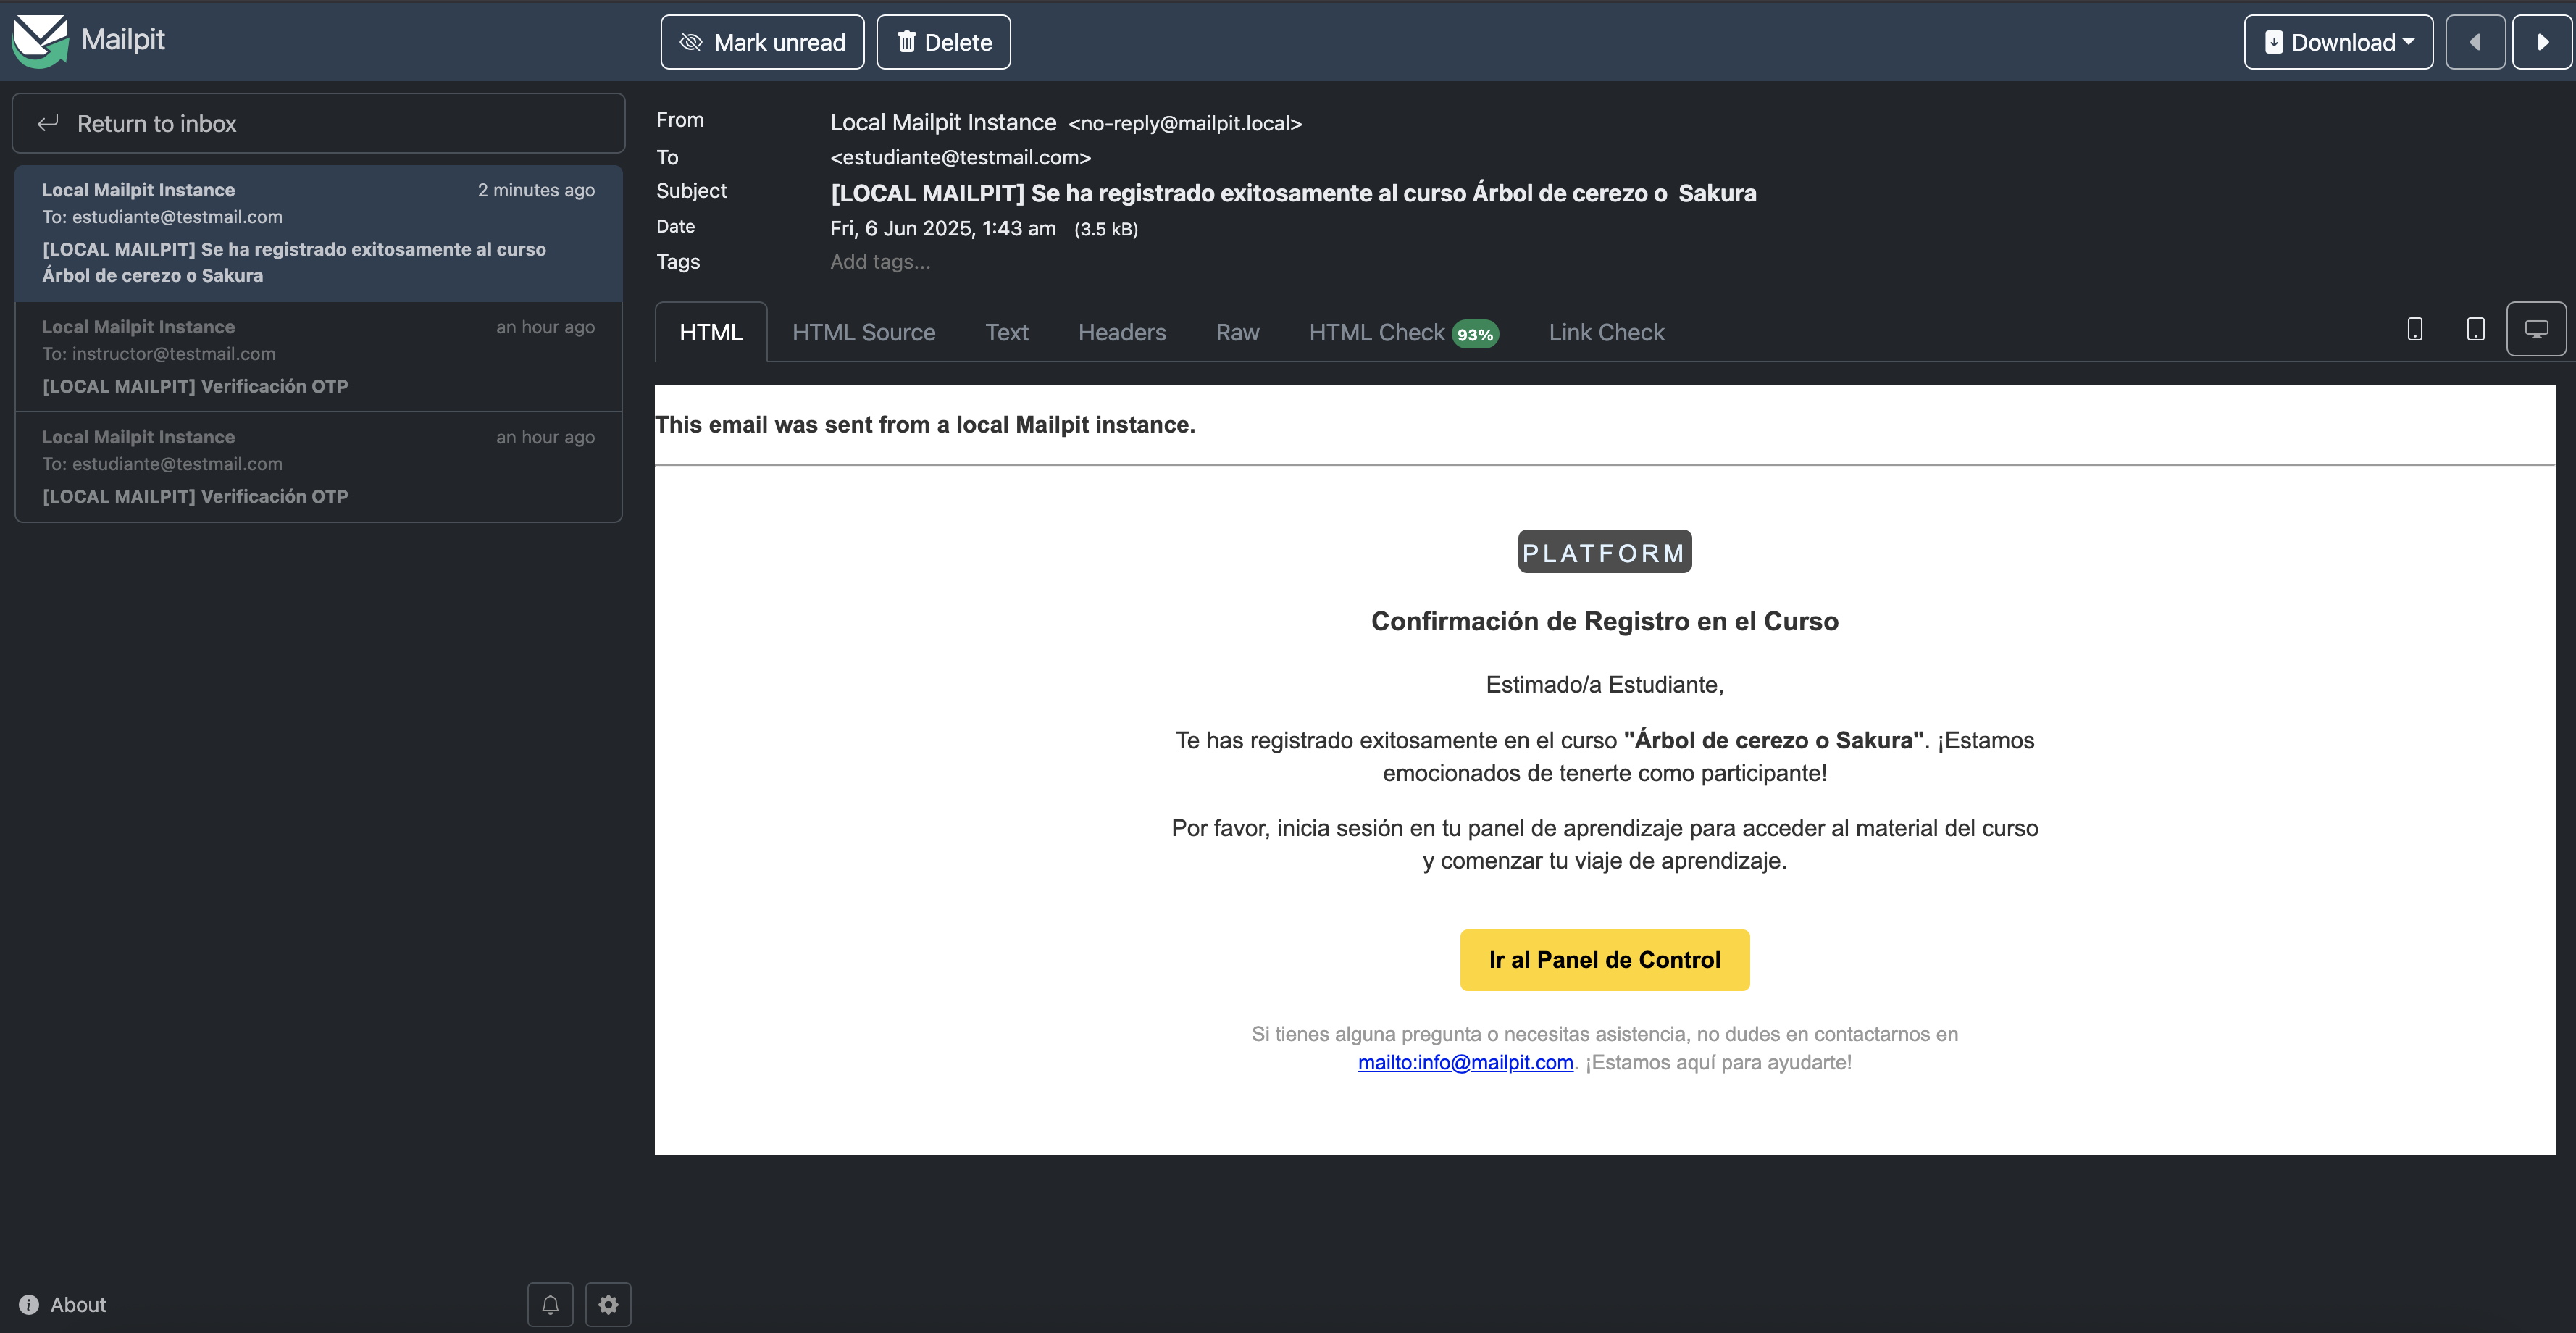
\includegraphics[width=\linewidth]{mail/mail_02.png}
    \caption{Correo de confirmación de registro a curso}
    \label{fig:correo_electronico_confirmacion_registro_curso}
\end{figure}
